\chapter{Analisis}
\label{chap:analisis}

\section{Analisis Portal Akademik Mahasiswa}
Portal Akademik Mahasiswa merupakan sebuah situs jaringan yang diperuntukan bagi mahasiswa dalam rangka mendapatkan informasi kegiatan akademik\cite{BTI:2012}. Mahasiswa dapat mengakses Portal Akademik Mahasiswa melalui URL \url{https://studentportal.unpar.ac.id/}. Untuk mengakses Portal Akademik Mahasiswa, mahasiswa harus \textit{login} menggunakan akun email \textit{student}. Halaman \textit{login} Student Portal UNPAR terintegrasi dengan CAS (\textit{Central Authentication Service}) UNPAR\footnote{\url{https://cas.unpar.ac.id}}.

\begin{figure}[H]
	\centering
	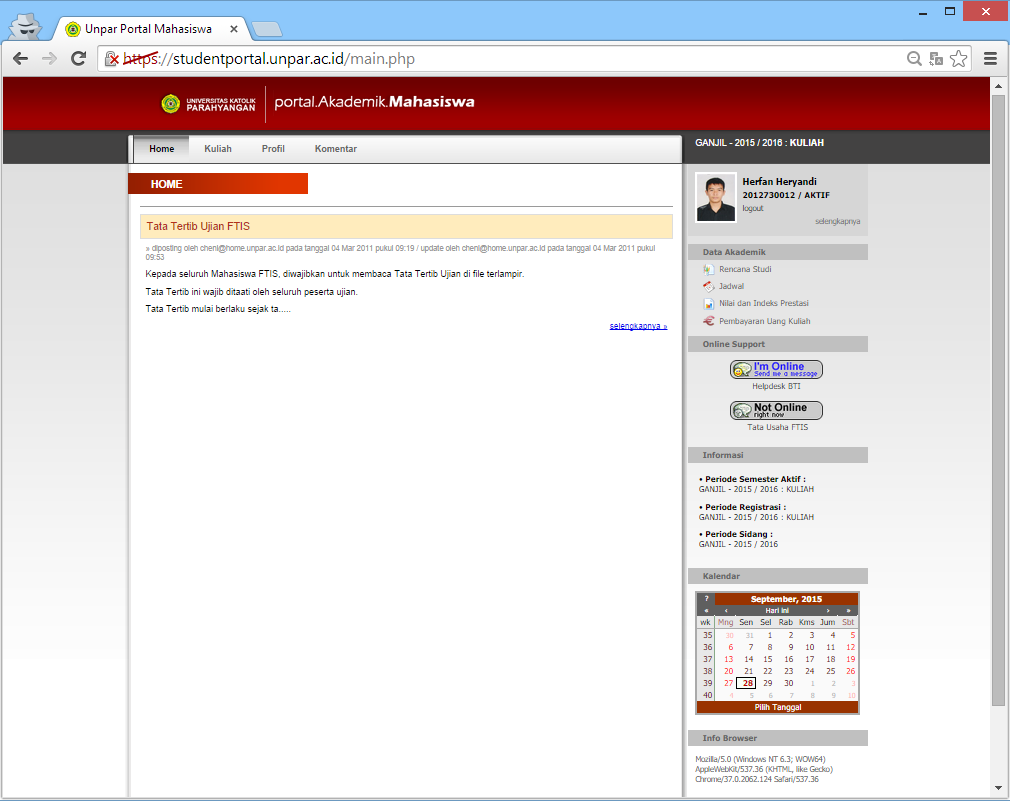
\includegraphics[scale=0.5]{Gambar/pam-home}
	\caption{Halaman Utama Portal Akademik Mahasiswa} 
	\label{fig:3_pam_home}
\end{figure}

Pada halaman utama Portal Akademik Mahasiswa (gambar \ref{fig:3_pam_home}), terdapat beberapa bagian yaitu:
\begin{enumerate}
	\item Menu Atas\\
	Menu ini berfungsi sebagai menu pendukung yang terdiri dari : 
	\begin{itemize}
		\item \textbf{Home}, menampilkan informasi atau pengumuman yang dikeluarkan oleh fakultas masing-masing (Gambar \ref{fig:3_pam_atas_home}). 
		
		\begin{figure}[H]
			\centering
			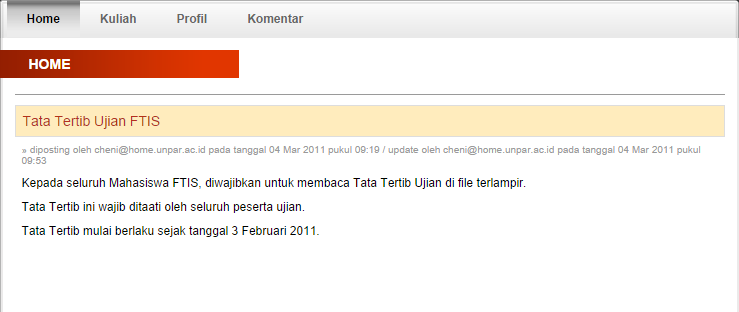
\includegraphics[scale=0.5]{Gambar/pam-atas-home}
			\caption{Menu Atas Home} 
			\label{fig:3_pam_atas_home}
		\end{figure}
		
		\item \textbf{Kuliah}, menampilkan pengumuman per mata kuliah sesuai dengan mata kuliah dan kelas yang diambil oleh masing-masing mahasiswa (Gambar \ref{fig:3_pam_atas_kuliah}).  
		
		\begin{figure}[H]
			\centering
			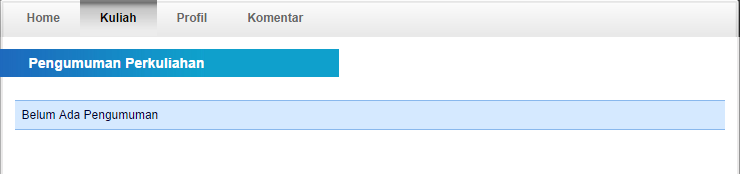
\includegraphics[scale=0.5]{Gambar/pam-atas-kuliah}
			\caption{Menu Atas Kuliah} 
			\label{fig:3_pam_atas_kuliah}
		\end{figure}
		
		\item \textbf{Profil}, berisi tentang data diri masing-masing mahasiswa (Gambar \ref{fig:3_pam_atas_profil}). 
		
		\begin{figure}[H]
			\centering
			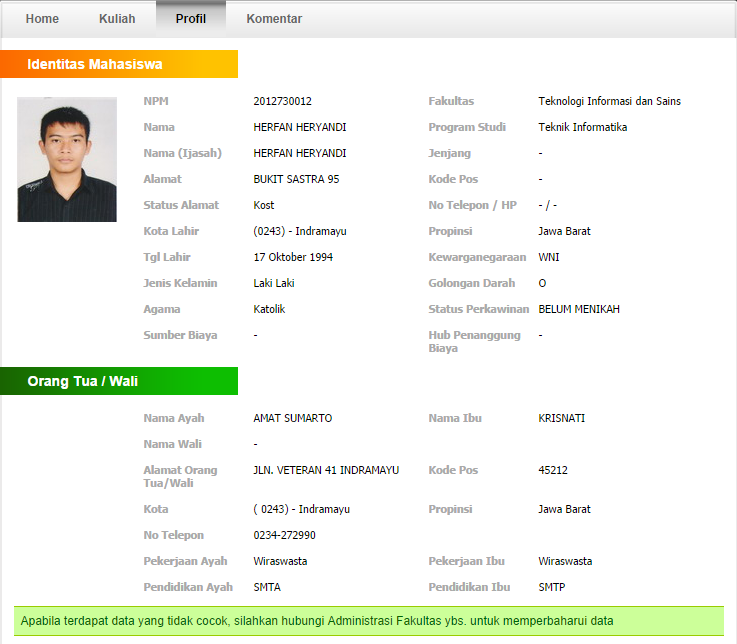
\includegraphics[scale=0.5]{Gambar/pam-atas-profil}
			\caption{Menu Atas Profil} 
			\label{fig:3_pam_atas_profil}
		\end{figure}
		
		\item \textbf{Komentar}, berisi komentar, saran, dan kritik dari mahasiswa (Gambar \ref{fig:3_pam_atas_komentar}).
		
		\begin{figure}[H]
			\centering
			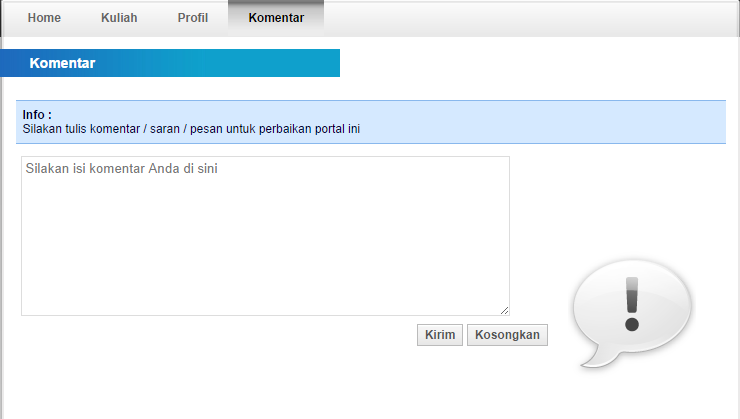
\includegraphics[scale=0.5]{Gambar/pam-atas-komentar}
			\caption{Menu Atas Komentar} 
			\label{fig:3_pam_atas_komentar}
		\end{figure}

	\end{itemize}
	
	\item Identitas Portal \\
	Bagian ini menampilkan identitas pengguna portal. Tampilan identitas ini dapat ditampilkan lengkap dengan melakukan klik pada \textit{link} ``selengkapnya'' atau ditampilkan minimal dengan klik \textit{link} ``tutup''. Identitas yang ditampilkan adalah nama, Nomor Pokok Mahasiswa (NPM), status keaktifan, pas foto, email, dosen wali, program studi, dan fakultas seperti yang terlihat pada gambar \ref{fig:3_pam_identitas}.   
	\begin{figure}[H]
			\centering
			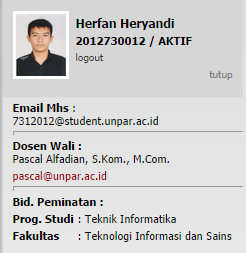
\includegraphics[scale=0.75]{Gambar/pam-identitas}
			\caption{Identitas Portal} 
			\label{fig:3_pam_identitas}
		\end{figure}
		
	\item Menu Utama\\
	Bagian ini memuat fitur utama Portal Akademik Mahasiswa mengenai data akademik (gambar \ref{fig:3_pam_utama}) yang terdiri dari:
		\begin{figure}[H]
			\centering
			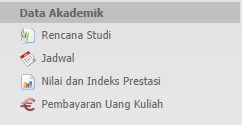
\includegraphics[scale=0.75]{Gambar/pam-utama}
			\caption{Menu Utama} 
			\label{fig:3_pam_utama}
		\end{figure}
	\begin{itemize}
	
		\item \textbf{Rencana Studi}\\
		Menu Rencana Studi terdiri dari submenu: 
		\begin{itemize}
			\item Registrasi (FRS/PRS)\\
			Digunakan sebagai formulir pengisian rencana studi awal (FRS) dan perubahan rencana studi (PRS) (Gambar \ref{fig:3_pam_utama_registrasi}). 			
			\begin{figure}[H]
				\centering
				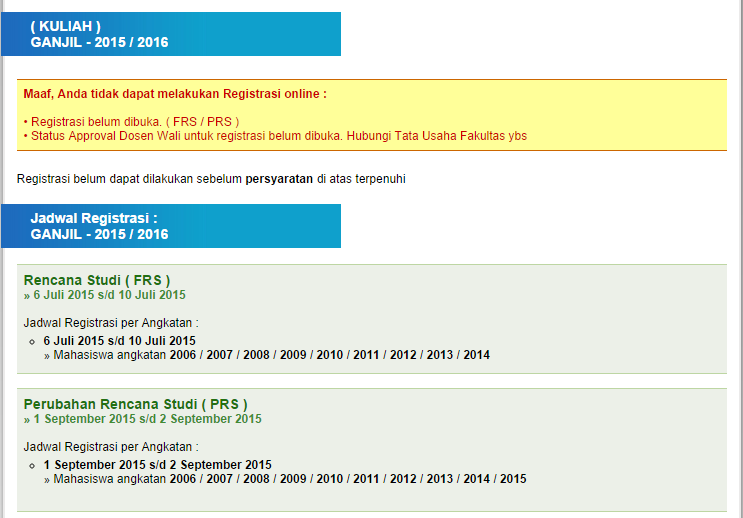
\includegraphics[scale=0.5]{Gambar/pam-utama-rencanastudi}
				\caption{Tampilan Registrasi FRS/PRS} 
				\label{fig:3_pam_utama_registrasi}
			\end{figure}
			
			\item Kartu Rencana Studi \\
			Menampilkan informasi mata kuliah yang telah diambil melalui submenu Registrasi (Gambar \ref{fig:3_pam_utama_krs}). Kartu Rencana Studi juga dapat dicetak melalui submenu ini. 
			\begin{figure}[H]
				\centering
				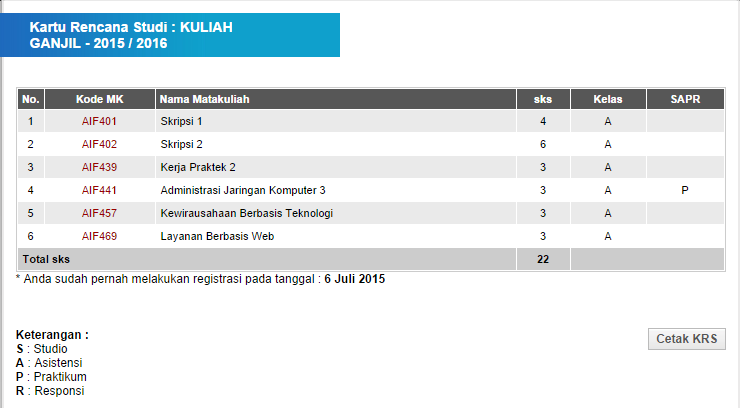
\includegraphics[scale=0.5]{Gambar/pam-utama-krs}
				\caption{Tampilan Kartu Rencana Studi\cite{BTI:2012}} 
				\label{fig:3_pam_utama_krs}
			\end{figure}
			
			\item Pindah Kelas MKU \\
			Mahasiswa dapat memilih kelas yang masih tersedia di kolom Jadwal Baru dan menekan tombol ``Simpan'' untuk setiap kelas yang diubah (Gambar \ref{fig:3_pam_utama_pindahmku}). 
			\begin{figure}[H]
				\centering
				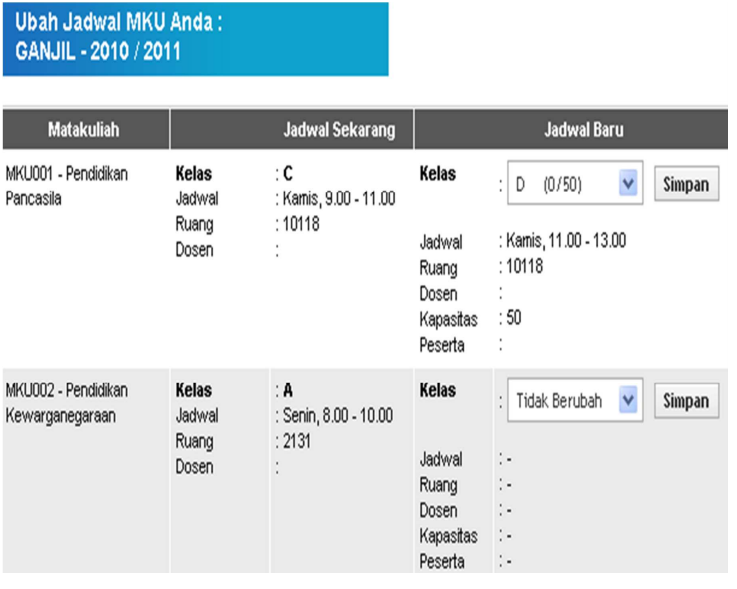
\includegraphics[scale=0.5]{Gambar/pam-utama-pindahmku}
				\caption{Tampilan Pindah Kelas MKU\cite{BTI:2012}} 
				\label{fig:3_pam_utama_pindahmku}
			\end{figure}

		\end{itemize}
		
		\item \textbf{ Jadwal}\\
		Menu Jadwal terdiri dari submenu: 
		\begin{itemize}
			\item Kuliah, UTS, dan UAS \\
			Submenu ini berisi tentang jadwal kuliah, UTS dan UAS yang dapat disusun per semester (Gambar \ref{fig:3_pam_utama_jadwal}). 
			\begin{figure}[H]
				\centering
				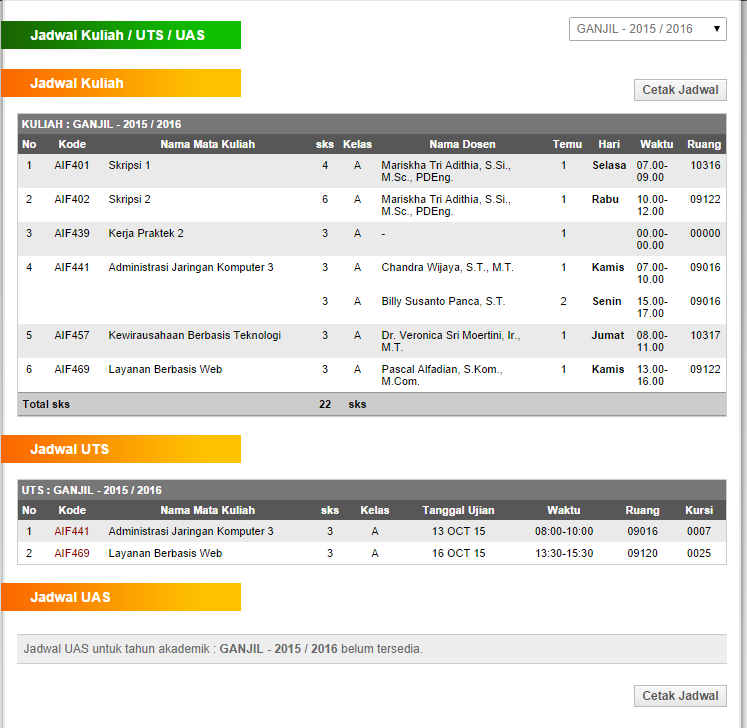
\includegraphics[scale=0.5]{Gambar/pam-utama-jadwal}
				\caption{Tampilan Jadwal Kuliah, UTS, dan UAS} 
				\label{fig:3_pam_utama_jadwal}
			\end{figure}
			
			\item MKU \\
			Submenu ini menampilkan seluruh jadwal Mata Kuliah Umum (MKU) yang memberikan informasi tentang kelas-kelas yang dibuka oleh Pusat Kajian Humaniora (PKH) (Gambar \ref{fig:3_pam_utama_jadwalmku}). 
			\begin{figure}[H]
				\centering
				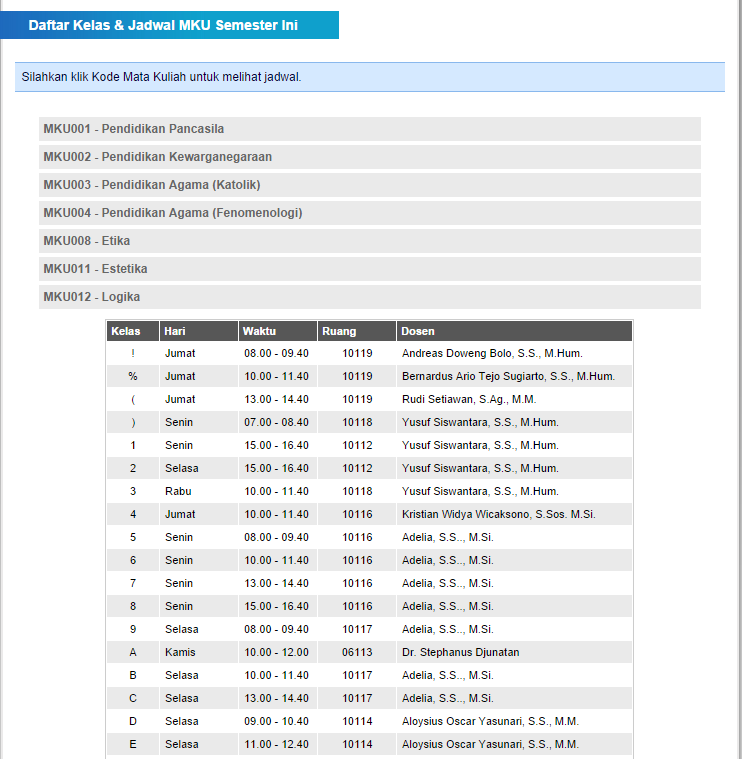
\includegraphics[scale=0.5]{Gambar/pam-utama-jadwalmku}
				\caption{Tampilan Jadwal MKU} 
				\label{fig:3_pam_utama_jadwalmku}
			\end{figure}
			
			\item Seluruh Fakultas \\
			Fitur ini memberikan informasi mengenai jadwal-jadwal yang ada di seluruh fakultas (Gambar \ref{fig:3_pam_utama_jadwalall}).
			\begin{figure}[H]
				\centering
				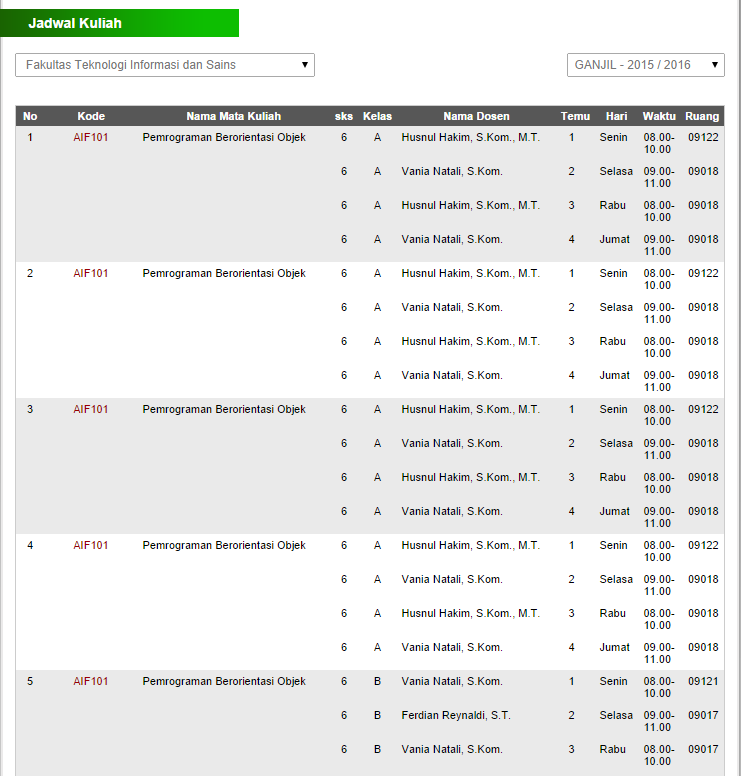
\includegraphics[scale=0.5]{Gambar/pam-utama-jadwalall}
				\caption{Tampilan Jadwal Seluruh Fakultas} 
				\label{fig:3_pam_utama_jadwalall}
			\end{figure}
		\end{itemize}
		
		\item \textbf{Nilai dan Indeks Prestasi}\\
		Menu Nilai dan Indeks Prestasi terdiri dari submenu: 
		\begin{itemize}
			\item Riwayat per Semester \\
			Submenu ini menampilkan informasi nilai per semester. Mahasiswa dapat melihat nilai sesuai dengan semester yang dipilih atau bisa memilih
pilihan ``Seluruh Tahun Akademik'' untuk melihat seluruh nilai berdasarkan semester (Gambar \ref{fig:3_pam_utama_nilai}).
			\begin{figure}[H]
				\centering
				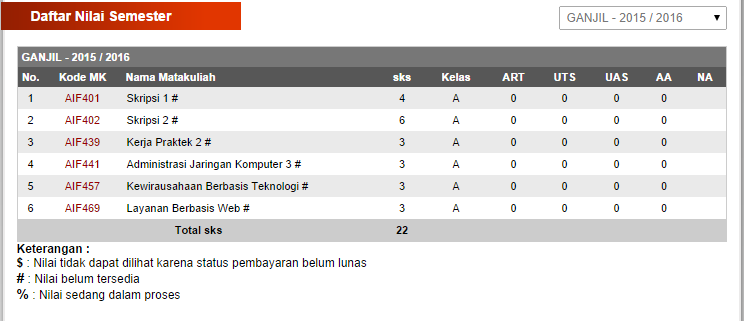
\includegraphics[scale=0.5]{Gambar/pam-utama-nilai}
				\caption{Tampilan Riwayat Per Semester} 
				\label{fig:3_pam_utama_nilai}
			\end{figure}
			
			\item Daftar Perkembangan Studi \\
			Seluruh riwayat mata kuliah dan nilai yang pernah ditempuh ditampilkan di submenu ini (Gambar \ref{fig:3_pam_utama_dps}). Pada bagian bawah halaman, terdapat statistik nilai dan indeks prestasi (Gambar \ref{fig:3_pam_utama_dpsstat}). 
			\begin{figure}[H]
				\centering
				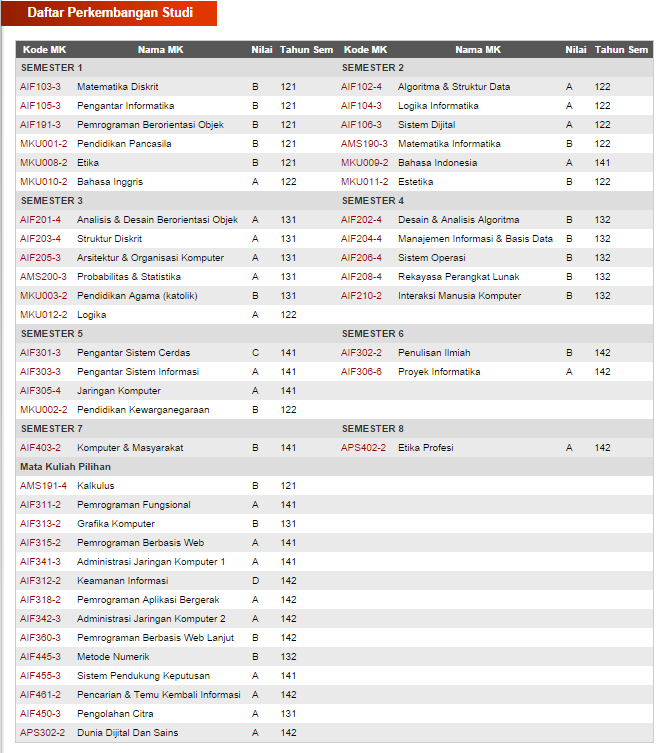
\includegraphics[scale=0.5]{Gambar/pam-utama-dps}
				\caption{Tampilan Daftar Perkembangan Studi} 
				\label{fig:3_pam_utama_dps}
			\end{figure}
			
			\begin{figure}[H]
				\centering
				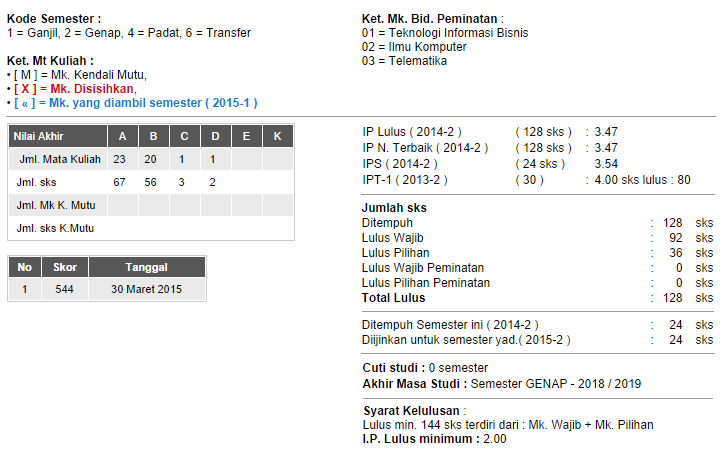
\includegraphics[scale=0.5]{Gambar/pam-utama-dpsstat}
				\caption{Tampilan Statistik Nilai dan IP} 
				\label{fig:3_pam_utama_dpsstat}
			\end{figure}
			
			\item Riwayat Indeks Prestasi \\
			Menampilkan daftar riwayat indeks prestasi semester dan kumulatif setiap semester. Tampilan ini juga dilengkapi dengan grafik perkembangan (Gambar \ref{fig:3_pam_utama_ip}). 
			\begin{figure}[H]
				\centering
				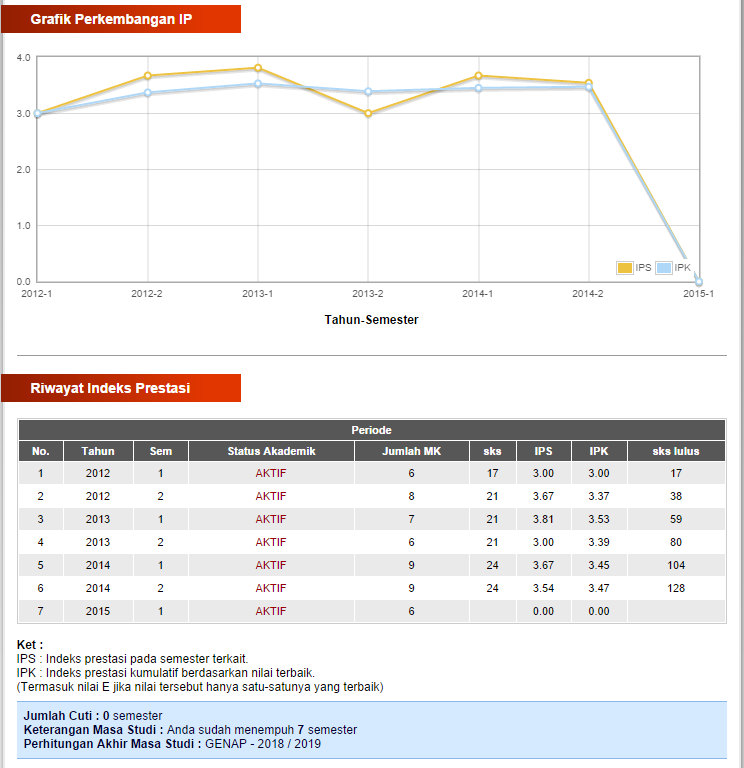
\includegraphics[scale=0.5]{Gambar/pam-utama-ip}
				\caption{Tampilan Riwayat Indeks Prestasi} 
				\label{fig:3_pam_utama_ip}
			\end{figure}
			
			\item TOEFL \\
			Menampilkan daftar riwayat skor \textit{Test of English as Foreign Language} (TOEFL) yang pernah ditempuh (Gambar \ref{fig:3_pam_utama_toefl}). Mahasiswa diwajibkan untuk menempuh TOEFL dengan skor minimal 500.
			
			\begin{figure}[H]
				\centering
				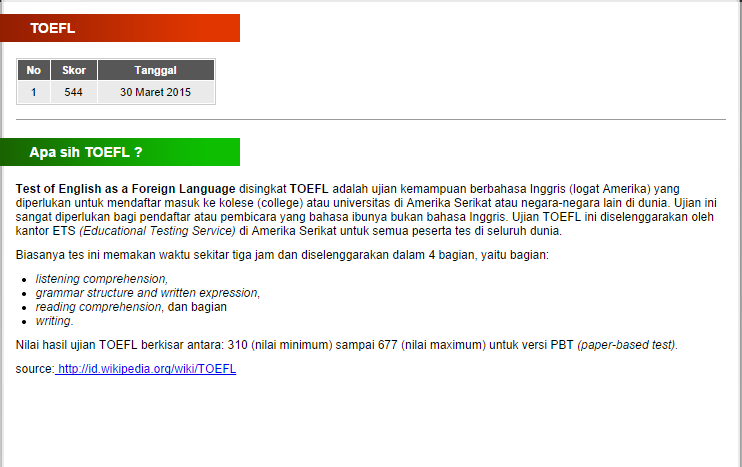
\includegraphics[scale=0.5]{Gambar/pam-utama-toefl}
				\caption{Tampilan TOEFL} 
				\label{fig:3_pam_utama_toefl}
			\end{figure}
		\end{itemize}
		
		\item \textbf{Pembayaran Uang Kuliah}\\
		Menu ini berfungsi untuk melihat data tagihan pembayaran uang kuliah serta cara-cara pembayarannya (Gambar \ref{fig:3_pam_utama_pembayaran}).
		\begin{figure}[H]
				\centering
				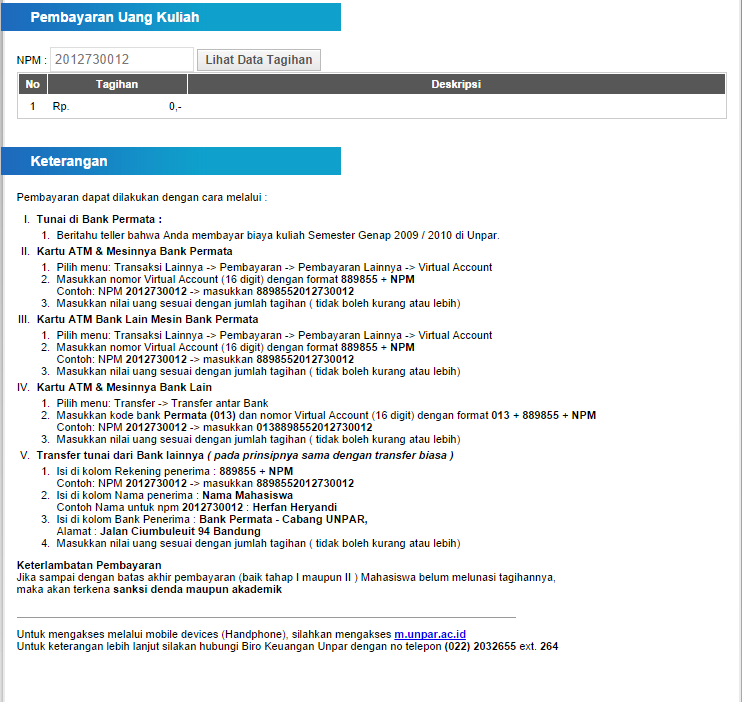
\includegraphics[scale=0.5]{Gambar/pam-utama-pembayaran}
				\caption{Tampilan Pembayaran Uang Kuliah} 
				\label{fig:3_pam_utama_pembayaran}
			\end{figure}
		\end{itemize}
		
	\item \textbf{Informasi}\\
		Bagian ini menampilkan informasi tentang periode-periode yang sedang aktif (Gambar \ref{fig:3_pam_utama_informasi}). Sebagai contoh jika ``Periode Registrasi'' diklik maka akan muncul \textit{pop up} seperti pada gambar \ref{fig:3_pam_utama_informasipop}.
			\begin{figure}[H]
				\centering
				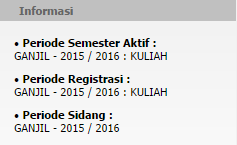
\includegraphics[scale=0.75]{Gambar/pam-utama-informasi}
				\caption{Tampilan Informasi} 
				\label{fig:3_pam_utama_informasi}
			\end{figure}
			
			\begin{figure}[H]
				\centering
				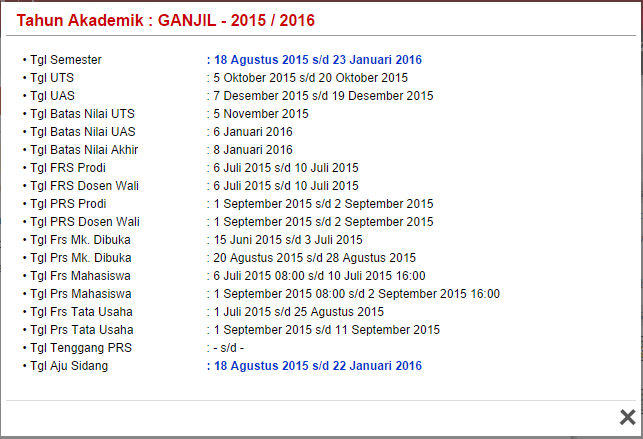
\includegraphics[scale=0.5]{Gambar/pam-utama-infopop}
				\caption{Tampilan \textit{Pop Up} Informasi} 
				\label{fig:3_pam_utama_informasipop}
			\end{figure}
		
	\item \textbf{Kalender}\\
		Bagian ini menampilkan kalender masehi (Gambar \ref{fig:3_pam_utama_kalender}).
		\begin{figure}[H]
				\centering
				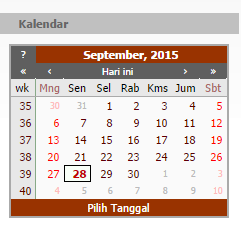
\includegraphics[scale=0.75]{Gambar/pam-utama-kalender}
				\caption{Tampilan Kalender} 
				\label{fig:3_pam_utama_kalender}
			\end{figure}
		
	\item \textbf{Info Browser}\\
		Bagian ini menampilkan informasi tentang internet \textit{browser} yang digunakan pada saat membuka Portal Akademik Mahasiswa (Gambar \ref{fig:3_pam_utama_infobrowser}). 
		\begin{figure}[H]
				\centering
				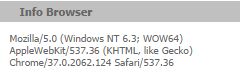
\includegraphics[scale=0.75]{Gambar/pam-utama-infobrowser}
				\caption{Tampilan Info Browser} 
				\label{fig:3_pam_utama_infobrowser}
			\end{figure}
\end{enumerate}

\section{Analisis Kebutuhan Informatika Student Portal}
\label{sec:kebutuhan}
Dalam menganalisis kebutuhan Informatika Student Portal, penulis melakukan wawancara dengan mahasiswa Program Studi Teknik Informatika UNPAR. Sampel yang diambil adalah lima orang mahasiswa dari setiap angkatan dalam empat tahun terakhir yaitu angkatan 2012 sampai 2015. Setelah melakukan wawancara, penulis memperoleh fitur-fitur yang diinginkan mahasiswa antara lain:
\begin{enumerate}
	\item Prasyarat mata kuliah\\
	Mahasiswa bisa memeriksa prasyarat mata kuliah saat FRS sehingga tidak terjadi kesalahan pengambilan mata kuliah. Prasyarat mata kuliah yang ditampilkan di Portal Akademik Mahasiswa kurang akurat. Selain itu, dari 20 mahasiswa yang diwawancara, hanya ada satu mahasiswa yang mengetahui bahwa Portal Akademik Mahasiswa memiliki fitur prasyarat. Prasyarat mata kuliah untuk Program Studi Teknik Informatika juga tersedia di \url{http://tinyurl.com/lionov}\footnote{\url{http://tinyurl.com/lionov}, diakses 5 September 2015}, namun mahasiswa merasa kurang praktis karena harus memeriksa secara manual. Mahasiswa menginginkan agar fitur ini bisa dibuat untuk mempermudah FRS. Fitur ini akan menampilkan seluruh mata kuliah yang dibuka beserta status pengambilannya.
	\item Ringkasan data akademik\\
	Ringkasan data akademik menampilkan data mengenai mata kuliah pilihan wajib dan sisa SKS untuk mencapai kelulusan. Mahasiswa menginginkan fitur ini dibuat untuk membantu mereka dalam mengatur perkuliahannya.
	\item Perubahan IPS dan IPK berdasarkan riwayat nilai\\
	Dalam Portal Akademik Mahasiswa, nilai pertama kali muncul dalam riwayat nilai. Riwayat IP tidak berubah secara otomatis saat seluruh nilai di riwayat nilai sudah muncul. Mahasiswa menginginkan agar IPS dan IPK dapat berubah secara otomatis saat nilai muncul.
	\item Jadwal kuliah yang tersusun\\
	Tampilan jadwal kuliah dalam Portal Akademik Mahasiswa tidak terurut berdasarkan hari seperti pada gambar \ref{fig:3_jadwal_portal} sehingga perlu direkapitulasi lagi. Mahasiswa menginginkan agar tampilan jadwal tersusun dan dalam bentuk seperti gambar \ref{fig:3_jadwal_rekap}.
		\begin{figure}[H]
			\centering
			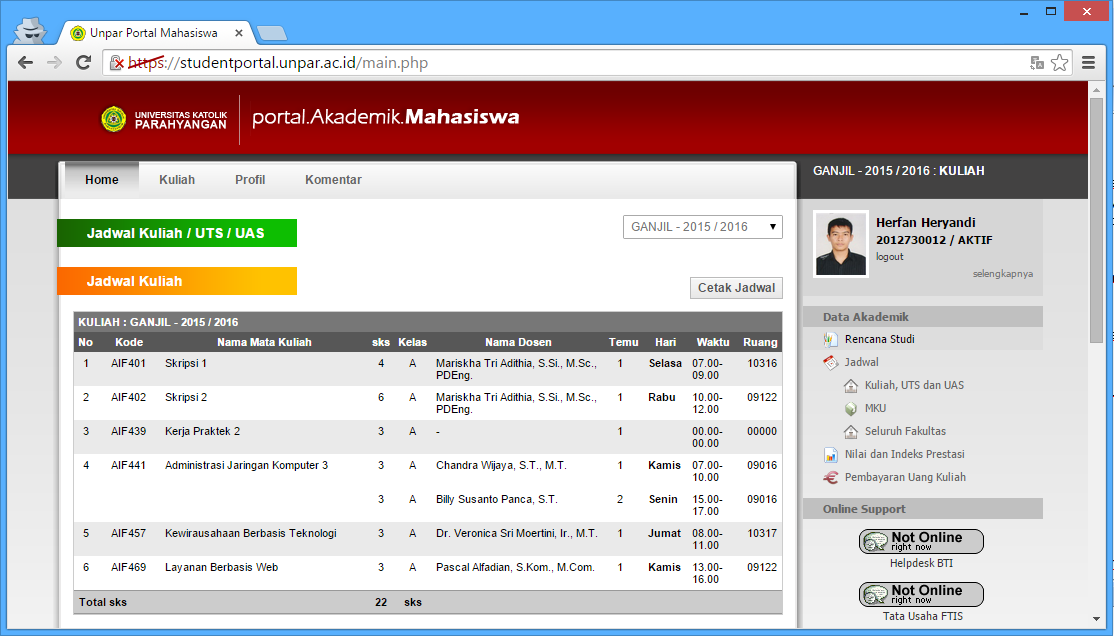
\includegraphics[scale=0.5]{Gambar/jadwal-portal}
			\caption{Tampilan Jadwal pada Portal Akademik Mahasiswa} 
			\label{fig:3_jadwal_portal}
		\end{figure}
		
		\begin{figure}[H]
			\centering
			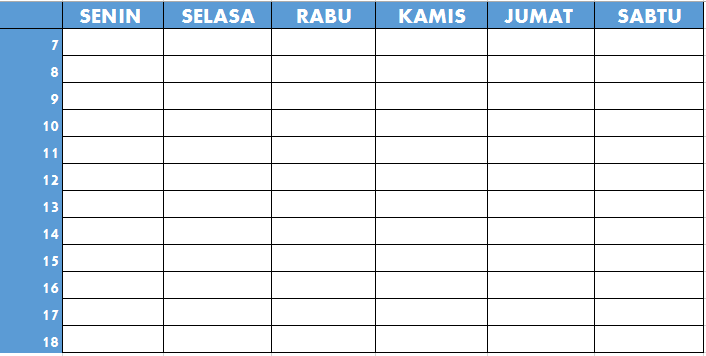
\includegraphics[scale=0.5]{Gambar/jadwal-rekap}
			\caption{Tampilan Jadwal yang Diinginkan Mahasiswa} 
			\label{fig:3_jadwal_rekap}
		\end{figure}
		
	\item Kalender akademik\\
	Kalender akademik merupakan salah satu fitur pada Portal Akademik Mahasiswa namun sekarang fitur tersebut sudah tidak ada lagi. Mahasiswa menginginkan fitur kalender akademik kembali untuk mengetahui tanggal-tanggal penting pada perkuliahan. 
	\item Rincian pembayaran\\
	Tagihan pada Portal Akademik Mahasiswa tidak mencantumkan batas akhir pembayaran dan rincian nominal tagihan. Mahasiswa menginginkan rincian pembayaran agar tidak terlambat membayar uang kuliah dan dapat mengetahui rincian nominal tagihan.
	\item Rincian mata kuliah\\
	Setiap mata kuliah yang dibuka memiliki rincian seperti deskripsi mata kuliah dan jenis mata kuliah yaitu apakah mata kuliah tersebut wajib, pilihan, atau pilihan wajib. Mahasiswa menginginkan fitur ini agar dapat mengetahui mata kuliah apa yang akan dipelajari.
	\item Tampilan situs web sama di sistem operasi manapun\\
	Jika tidak menggunakan sistem operasi Windows seperti Linux dan Mac, saat mengakses Portal Akademik Mahasiswa melalui \url{https://studentportal.unpar.ac.id/}, maka mahasiswa akan diarahkan ke \url{https://m.studentportal.unpar.ac.id/} yaitu Portal Akademik Mahasiswa dengan tampilan \textit{mobile} (Gambar \ref{fig:3_pam_mobile}). Tampilan ini tidak memiliki fitur selengkap Portal Akademik Mahasiswa, hanya memiliki fitur pengumunan kuliah, jadwal kuliah, UTS, dan UAS, nilai, IP, dan tagihan. Selain itu, tampilan \textit{mobile} pada telepon seluler akan terlihat sangat kecil sehingga tidak sulit untuk memilih menu. Mahasiswa menginginkan fitur ini agar Informatika Student Portal dapat diakses di sistem operasi manapun tanpa perubahan tampilan.
	\begin{figure}[H]
			\centering
			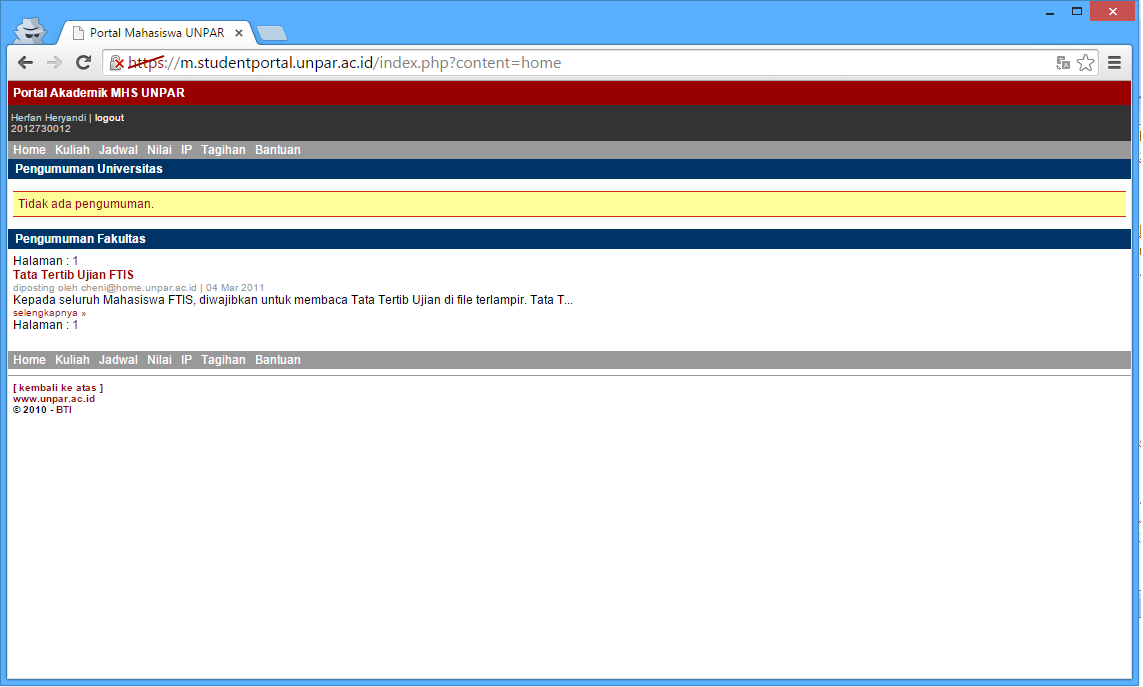
\includegraphics[scale=0.5]{Gambar/pam-mobile}
			\caption{Tampilan \textit{Mobile} Portal Akademik Mahasiswa} 
			\label{fig:3_pam_mobile}
		\end{figure}
	\item Kontak dosen\\
	Kontak dosen berisi informasi email setiap dosen sehingga dapat mempermudah mahasiswa untuk menghubungi dosen. Mahasiswa juga dapat mengirim email secara langsung melalui Portal Akademik Mahasiswa.
	\item Pohon kurikulum\\
	Mahasiswa munginnginkan agar dapat melihat pohon kurikulum Program Studi Teknik Informatika dalam Portal Akademik Mahasiswa.
	\item Pemberitahuan\\
	Mahasiswa menginginkan Portal Akademik Mahasiswa menampilkan pemberitahuan berupa \textit{pop up} mengenai pengumuman terkini.
	\item \textit{Chatting}\\
	Mahasiswa menginginkan agar dapat berkomunikasi dengan sesama pengguna Portal Akademik Mahasiswa melalui \textit{chat}.
	\item Unggah \textit{Curriculum Vitae}
	Mahasiswa menginginkan agar dapat mengunggah data mengenai kegiatan dan keaktifan di universitas agar dapat digunakan oleh perusahaan untuk mencari mahasiswa dengan kriteria tertentu misalnya untuk kepentingan magang dan beasiswa.
\end{enumerate}

Penulis menetapkan fitur-fitur yang akan dipilih untuk diimplementasikan harus memenuhi kriteria:
\begin{itemize}
	\item Data yang dibutuhkan dapat diambil dari Portal Akademik Mahasiwa \\
	Aplikasi Informatika Student Portal merupakan aplikasi hasil kustomisasi Portal Akademik Mahasiswa. Informasi yang ditampilkan Informatika Student Portal diperoleh dengan cara mengolah data dari Portal Akademik Mahasiswa. Jadi data yang dibutuhkan Informatika Student Portal harus dapat diambil dari Portal Akademik Mahasiswa. 
	\item Data hasil olahan tidak tersedia di Portal Akademik Mahasiswa\\
	Jika data hasil olahan yang sudah tersedia di Portal Akademik Mahasiswa, maka fitur tidak perlu dibuat lagi di Informatika Student Portal karena mahasiswa dapat mengakses langsung Portal Akademik Mahasiswa.
	\item Fitur mendukung fungsi Portal Akademik Mahasiswa sebagai sumber informasi akademik \\
	Portal Akademik Mahasiswa berfungsi sebagai sumber informasi akademik karena itu Informatika Student Portal juga harus mememiliki fitur yang dapat mendukung fungsi tersebut.
\end{itemize}

Hasil analisis fitur-fitur yang diinginkan berdasarkan kriteria di atas dan batas waktu pembangunan aplikasi dapat dilihat pada tabel \ref{tab:3_hasil_fitur}.
\begin{table}[H]
	\centering
		\caption{Tabel Hasil Analisis Kebutuhan Informatika Student Portal}
    \begin{tabular}{|p{4.5cm}|p{2.5cm}|p{8cm}|}
		\hline
		Fitur & Dibuat/Tidak dibuat & Alasan\\
		\hline
		Prasyarat mata kuliah                             & Dibuat       & Data dapat diambil dari Portal Akademik Mahasiswa dan aturan prasyarat mata kuliah Program Studi Teknik Informatika sudah tersedia di SIA Models                   \\
		\hline
    Ringkasan data akademik                               & Dibuat       & Data dapat diambil dari Portal Akademik Mahasiswa dan didukung oleh SIA Models                        \\
		\hline
    Perubahan IPS dan IPK berdasarkan riwayat nilai   & Dibuat       &  IPS dan IPK dapat dihitung melalui riwayat nilai yang dapat diperoleh dari Portal Akademik Mahasiswa \\
		\hline
    Jadwal kuliah yang tersusun                       & Dibuat       & Jadwal yang tersusun mempermudah mahasiswa untuk                                                      \\
		\hline
    Kalender akademik                                 & Tidak dibuat & Data tidak bisa diperoleh dari Portal Akademik Mahasiwa                                               \\
		\hline
    Rincian pembayaran                                & Tidak dibuat & Data tidak bisa diperoleh dari Portal Akademik Mahasiwa                                               \\
		\hline
    Rincian mata kuliah                               & Tidak dibuat & Data tidak bisa diperoleh dari Portal Akademik Mahasiwa                                               \\
		\hline
    Tampilan situs web sama di sistem operasi manapun & Dibuat       & Aplikasi yang akan dibuat merupakan situs web yang responsif                                          \\
		\hline
    Kontak dosen                                      & Tidak dibuat & Data tidak bisa diperoleh dari Portal Akademik Mahasiwa                                               \\
		\hline
    Pemberitahuan                                     & Tidak dibuat & Waktu pengerjaan yang terbatas                                                                        \\
		\hline
    Unggah \textit{Curriculum Vitae}                           & Tidak dibuat & Tidak mendukung Portal Akademik Mahasiswa sebagai sumber informasi akademik                           \\
		\hline
		\end{tabular}
	\label{tab:3_hasil_fitur}
\end{table}


\section{Analisis Komunikasi Portal Akademik Mahasiswa untuk Fitur Informatika Student Portal}
Untuk memenuhi fitur Informatika Student Portal, peneliti menganalisis komunikasi Portal Akademik Mahasiswa ke dalam beberapa kasus yang akan dijelaskan pada subbab-subbab berikut.

\subsection{Kasus \textit{Login}}
Di Portal Akademik Mahasiswa, mahasiswa dapat \textit{login} dengan cara:
\begin{enumerate}
	\item Mengakses \url{https://studentportal.unpar.ac.id/} dan mengklik tombol ``input\#submit.login-button'' (Gambar \ref{fig:3_case_login}).
	\begin{figure}[H]
			\centering
			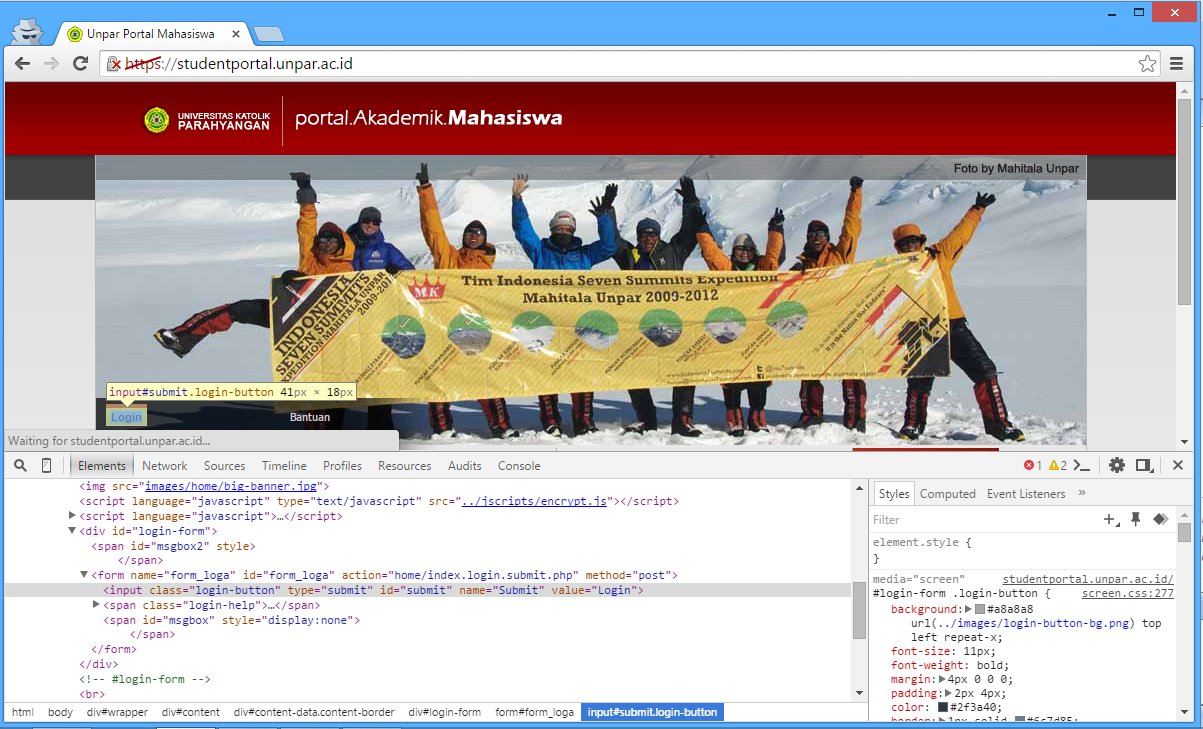
\includegraphics[scale=0.5]{Gambar/case-login}
			\caption{Tombol ``input\#submit.login-button'' pada Halaman Depan Portal Akademik Mahasiswa} 
			\label{fig:3_case_login}
		\end{figure}
		
	\item Saat tombol tersebut ditekan, mahasiswa akan dibawa ke halaman \url{index.login.submit.php} dengan \textit{form data} berisi:
			\begin{itemize}
				\item Submit: selalu berisi ``Login''
			\end{itemize}
		
	\item Secara otomatis halaman akan berpindah lagi ke \url{https://cas.unpar.ac.id/login? service=https\%3A\%2F\%2Fstudentportal.unpar.ac.id\%2Fhome\%2Findex.login.submit.php}.
		
	\item Di sana, akan ditampilkan halaman \textit{login} CAS UNPAR di mana mahasiswa diminta mengisi \textit{``Username''} pada kolom ``input\#username.required'' dan \textit{``Password''} pada kolom ``input\#password.required'' (Gambar \ref{fig:3_case_login_cas}).
	\begin{figure}[H]
			\centering
			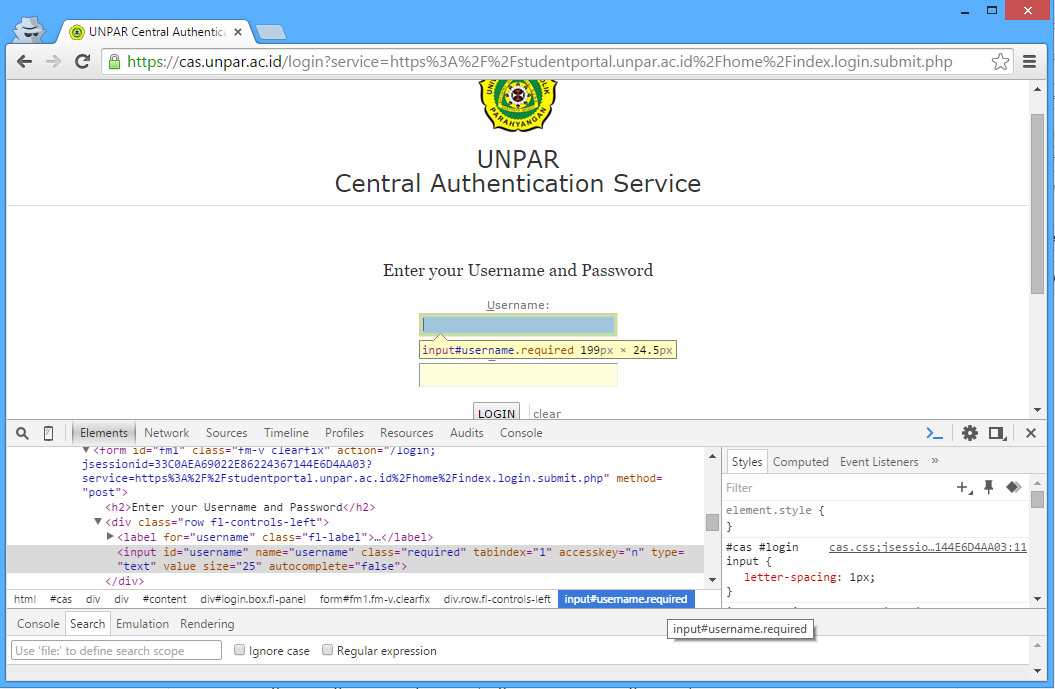
\includegraphics[scale=0.5]{Gambar/case-login-cas}
			\caption{Kolom \textit{``Username''} ``input\#username.required'' pada Halaman CAS UNPAR} 
			\label{fig:3_case_login_cas}
		\end{figure}
	\item Setelah itu mahasiswa harus menekan tombol ``input.btn-submit''. Data tersebut akan dikirimkan ke \url{/login;jsessionid=...?service=https://studentportal.unpar.ac.id/home/index.login.submit.php} dengan \textit{cookie}:
	\begin{itemize}
		\item JSESSIONID: diambil dari \textit{cookie} yang di-\textit{set} pada halaman \url{https://cas.unpar.ac.id/login? service=https\%3A\%2F\%2Fstudentportal.unpar.ac.id\%2Fhome\%2Findex.login.submit.php}
	\end{itemize}
	 Data yang dikirim juga mengandung \textit{form data} sebagai berikut (Gambar \ref{fig:3_case_form}):
	\begin{itemize}
		\item username: diambil dari nilai elemen ``input\#username.required''
		\item password: diambil dari nilai elemen ``input\#password.required''
		\item lt: diambil dari nilai elemen ``input'' dengan nama ``lt''
		\item execution: diambil dari nilai elemen ``input'' dengan nama ``execution''
		\item \_eventId: selalu berisi ``submit''
		\item submit: selalu berisi ``LOGIN''
		\begin{figure}[H]
			\centering
			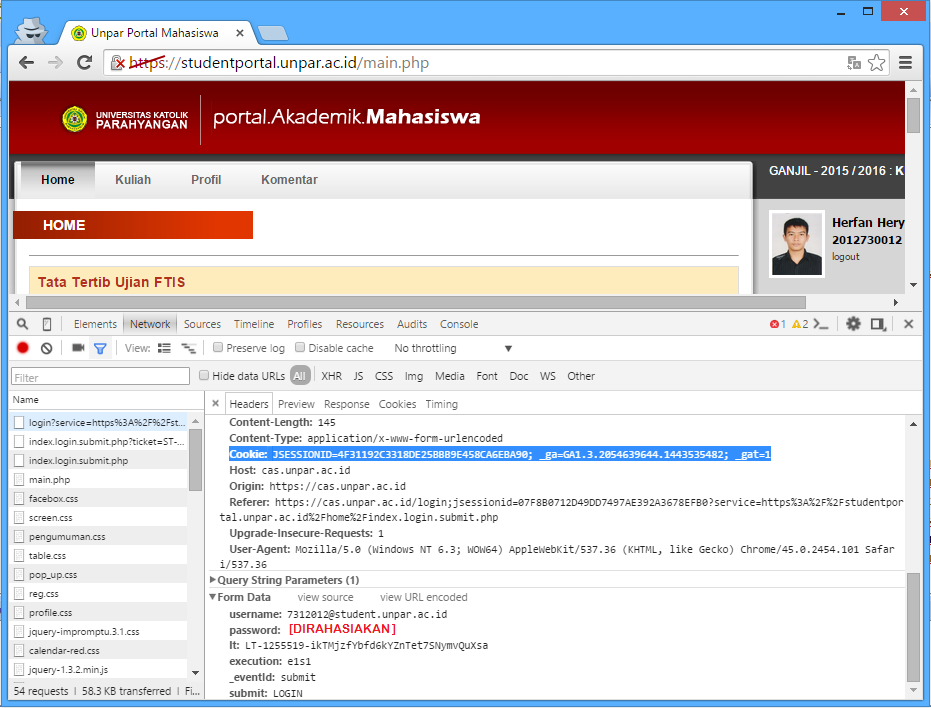
\includegraphics[scale=0.5]{Gambar/case-form}
			\caption{\textit{Form Data} yang dikirim CAS UNPAR} 
			\label{fig:3_case_form}
		\end{figure}
	\end{itemize}
\item Jika berhasil, akan dilakukan pengalihan beberapa kali dan diakhiri di \url{https://studentportal.unpar.ac.id/main.php} dengan \textit{cookie} sebagai berikut:
\begin{itemize}
	\item PHPSESSID: diambil dari \textit{cookie} yang di-\textit{set} pada beberapa pengalihan sebelumnya
	\item \_ga dan \_gat: tidak diperlukan, digunakan oleh Google Analytics\footnote{\url{https://developers.google.com/analytics/devguides/collection/analyticsjs/cookie-usage}}
\end{itemize}
\end{enumerate}

\subsection{Kasus Nilai}
Di halaman utama Portal Akademik Mahasiswa, mahasiswa dapat melihat riwayat nilai dengan cara:
\begin{enumerate}
	\item Mengklik ``a.first-line-menu'' dengan teks ``Nilai dan Indeks Prestasi'' 
	\item Setelah diklik, akan muncul list ``ul.hidden'', kemudian mahasiswa harus mengklik elemen ``a'' dengan teks ``Riwayat Per Semester'' (Gambar \ref{fig:3_case_nilai_menu})
	\begin{figure}[H]
			\centering
			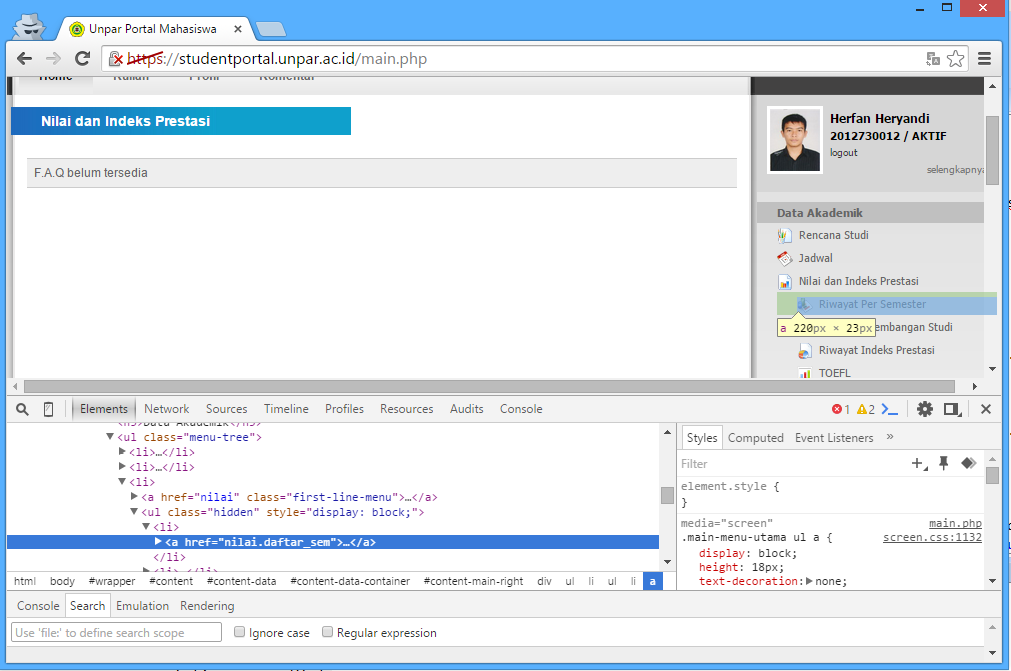
\includegraphics[scale=0.5]{Gambar/case-nilai-menu}
			\caption{Elemen ``a'' dengan teks ``Riwayat Per Semester'' pada Menu Nilai dan Indeks Prestasi} 
			\label{fig:3_case_nilai_menu}
		\end{figure}
		\item Setelah mengklik ``Riwayat Per Semester'', mahasiswa akan diarahkan ke \url{https://studentportal.unpar.ac.id/includes/nilai.daftar_sem.php} dengan \textit{cookie} sebagai berikut:
\begin{itemize}
	\item PHPSESSID: diambil dari \textit{cookie} yang di-\textit{set} saat pengalihan ke halaman utama
\end{itemize}
		\item Halaman ``Riwayat Per Semester'' menampilkan nilai semester terkini. Jika ingin melihat nilai semester sebelumnya, mahasiswa dapat mengklik \textit{combo box} ``select\#tahun\_akd\_sec'' kemudian memilih ``option'' yang diinginkan atau ``Seluruh Tahun Akademik'' untuk melihat nilai seluruh semester (Gambar \ref{fig:3_case_nilai_pilih}).
		
		\begin{figure}[H]
			\centering
			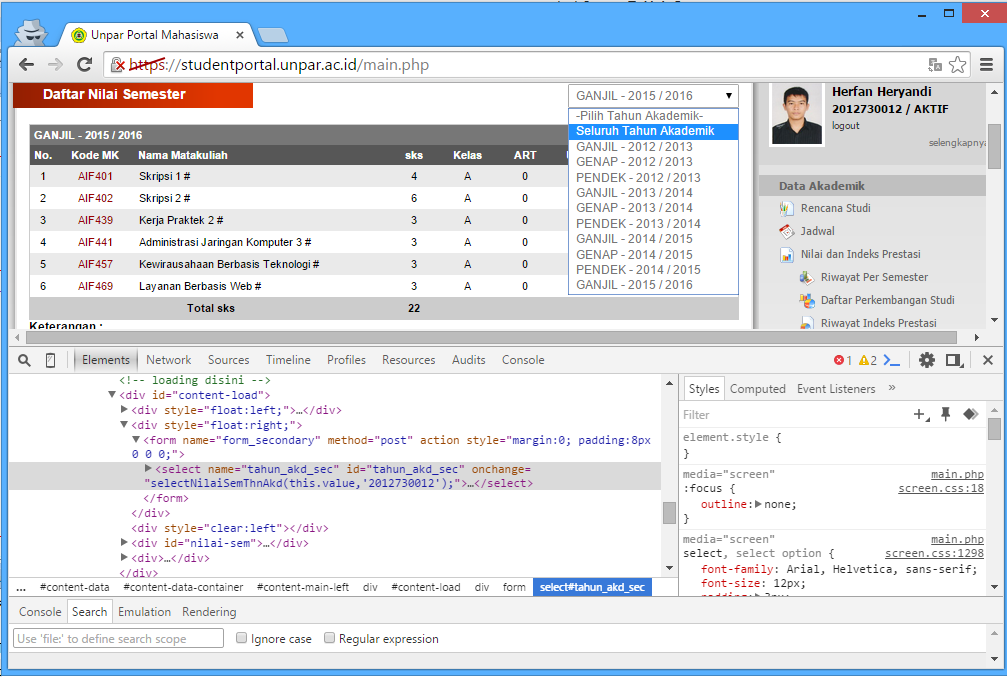
\includegraphics[scale=0.5]{Gambar/case-nilai-pilih}
			\caption{\textit{Combo Box} ``select\#tahun\_akd\_sec'' pada Halaman Riwayat Per Semester} 
			\label{fig:3_case_nilai_pilih}
		\end{figure}
		
		\item  Setelah memilih ``option'', mahasiswa akan dibawa ke \url{https://studentportal.unpar.ac.id/includes/nilai.sem.php} (Gambar \ref{fig:3_case_nilai}) dengan \textit{cookie} PHPSESSID dan mengandung \textit{form data}:
		\begin{itemize}
			\item npm: diperoleh dari NPM mahasiswa
			\item thn\_akd: berisi tahun akademik semester atau berisi ``ALL'' jika memilih ``Seluruh Tahun Akademik''
			\item sem\_akd: berisi semester akademik dalam angka (1: ganjil, 2: genap, 4: pendek) atau tidak didefinisikan jika memilih ``Seluruh Tahun Akademik''
		\end{itemize}
		
		\begin{figure}[H]
			\centering
			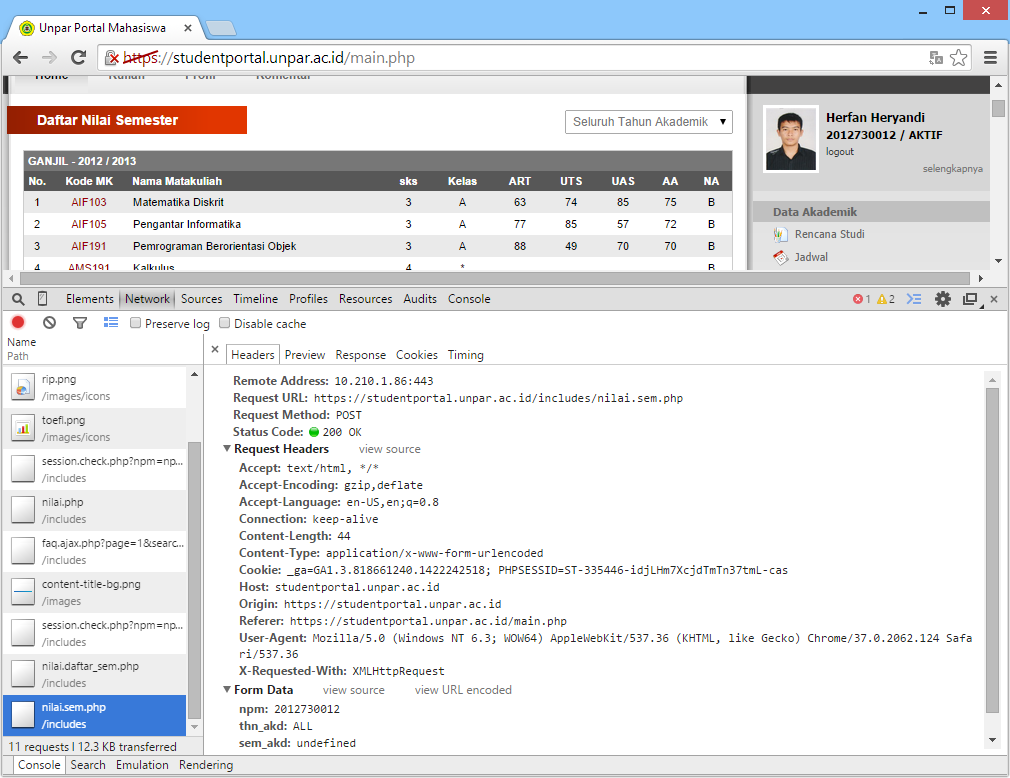
\includegraphics[scale=0.5]{Gambar/case-nilai}
			\caption{\textit{Form Data} pada pengiriman Nilai Seluruh Tahun Akademik} 
			\label{fig:3_case_nilai}
		\end{figure}
\end{enumerate}

\subsection{Kasus Jadwal}
Di halaman utama Portal Akademik Mahasiswa, mahasiswa dapat melihat jadwal dengan cara:
\begin{enumerate}
	\item Mengklik ``a.first-line-menu'' dengan teks ``Jadwal'' 
	\item Setelah diklik, akan muncul list ``ul.hidden'', kemudian mahasiswa harus mengklik elemen ``a'' dengan teks ``Kuliah, UTS dan UAS''(Gambar \ref{fig:3_case_jadwal_menu})
	\begin{figure}[H]
			\centering
			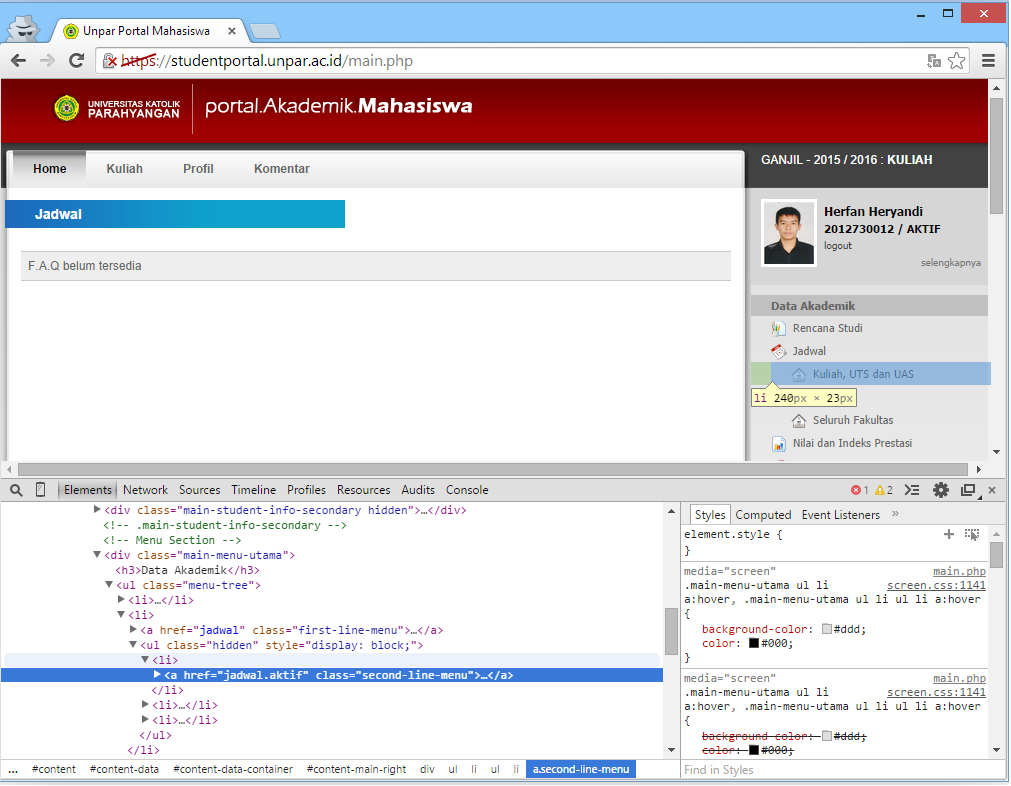
\includegraphics[scale=0.5]{Gambar/case-jadwal-menu}
			\caption{Elemen ``a'' dengan teks ``Kuliah, UTS dan UAS'' pada Menu Jadwal} 
			\label{fig:3_case_jadwal_menu}
		\end{figure}
		\item Setelah mengklik ``Kuliah, UTS dan UAS'', mahasiswa akan diarahkan ke \url{https://studentportal.unpar.ac.id/includes/jadwal.aktif.php} dengan \textit{cookie} sebagai berikut:
\begin{itemize}
	\item PHPSESSID: diambil dari \textit{cookie} yang di-\textit{set} saat pengalihan ke halaman utama
\end{itemize}
\item Halaman ``Kuliah, UTS dan UAS'' menampilkan jadwal kuliah, UTS, dan UAS semester terkini. Jika ingin melihat jadwal semester sebelumnya, mahasiswa dapat mengklik \textit{combo box} ``select\#tahun\_akd\_sec'' kemudian memilih ``option'' yang diinginkan (Gambar \ref{fig:3_case_jadwal_pilih}).
		
		\begin{figure}[H]
			\centering
			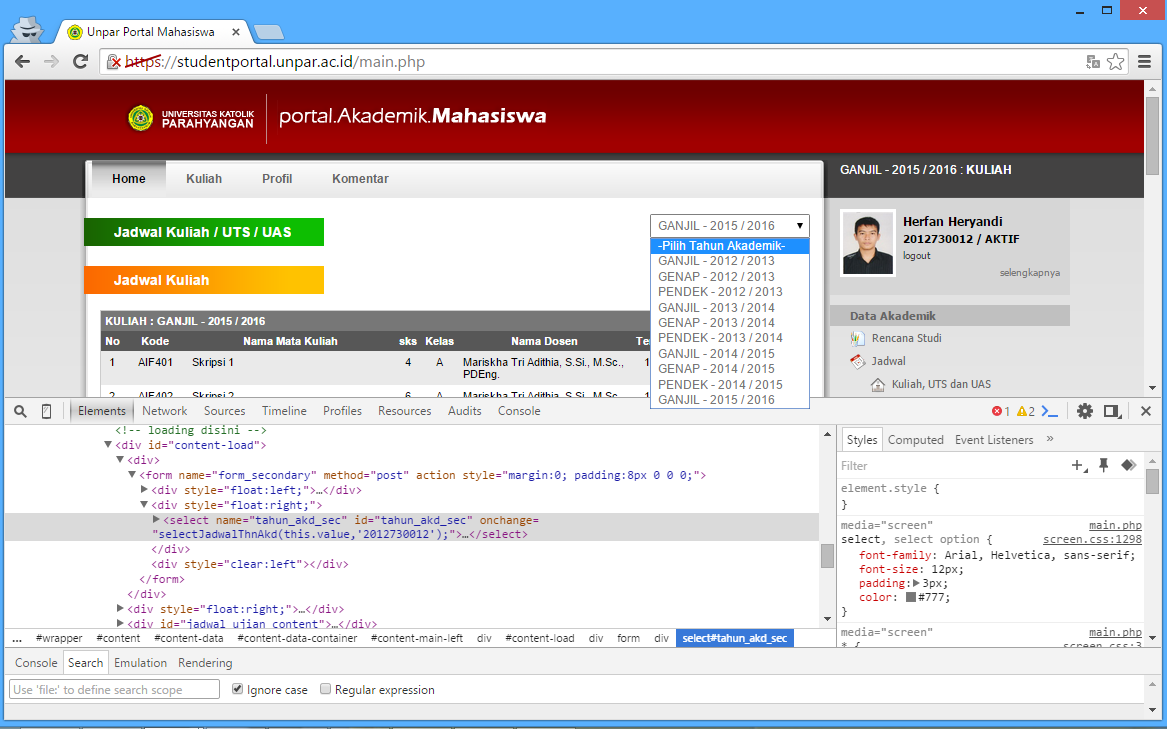
\includegraphics[scale=0.5]{Gambar/case-jadwal-pilih}
			\caption{Combo Box ``select\#tahun\_akd\_sec'' pada Halaman Jadwal Kuliah, UTS, dan UAS} 
			\label{fig:3_case_jadwal_pilih}
		\end{figure}
		
		\item  Setelah memilih ``option'', mahasiswa akan ditampilkan jawaban dari \url{https://studentportal.unpar.ac.id/includes/jadwal.kuliah.php} dan \url{https://studentportal.unpar.ac.id/includes/jadwal.ujian.php} (Gambar \ref{fig:3_case_jadwal}) dengan \textit{cookie} PHPSESSID dan mengandung \textit{form data}:
		\begin{itemize}
			\item npm: diperoleh dari NPM mahasiswa
			\item thn\_akd: berisi tahun akademik semester 
			\item sem\_akd: berisi semester akademik dalam angka (1: ganjil, 2: genap, 4: pendek) 
		\end{itemize}
		
		\begin{figure}[H]
			\centering
			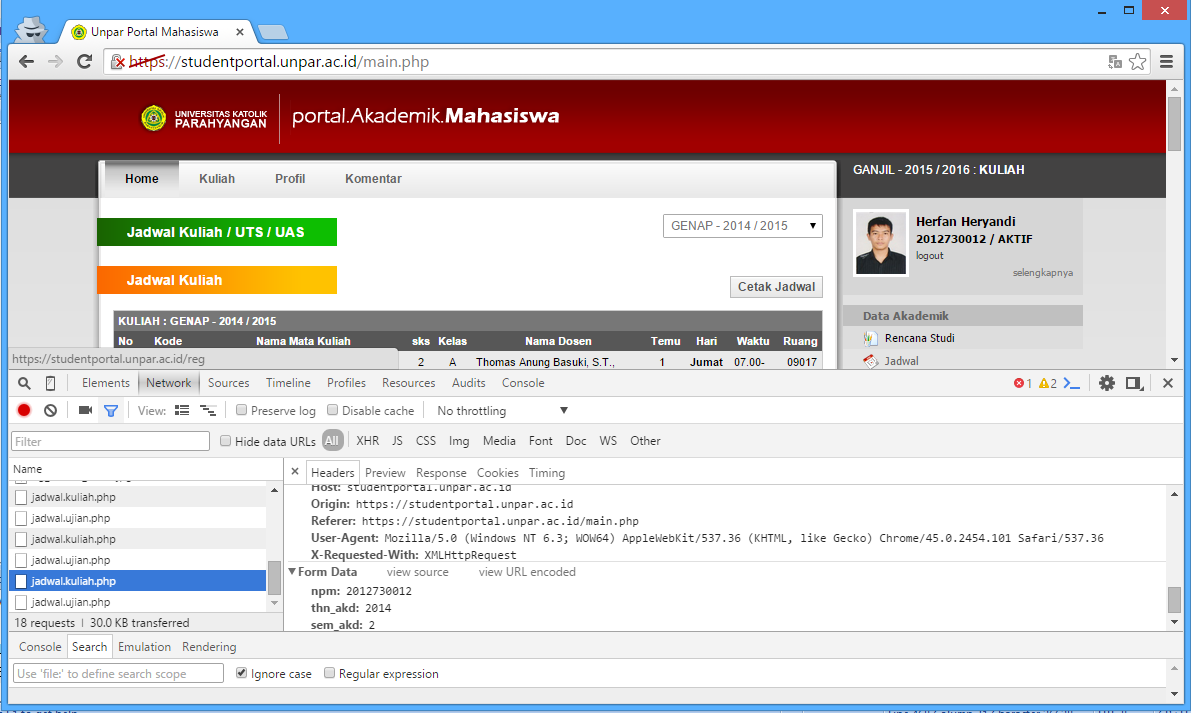
\includegraphics[scale=0.5]{Gambar/case-jadwal}
			\caption{\textit{Form Data} pada pengiriman Jadwal Kuliah dan Ujian} 
			\label{fig:3_case_jadwal}
		\end{figure}
		
\end{enumerate}

Mahasiswa juga dapat melihat jadwal seluruh fakultas dengan cara:
\begin{enumerate}
	\item Mengklik ``a.second-line-menu'' dengan teks ``Seluruh Fakultas'' pada \textit{list} ``ul.hidden'' (Gambar \ref{fig:3_case_jadwal_seluruh})
	\begin{figure}[H]
			\centering
			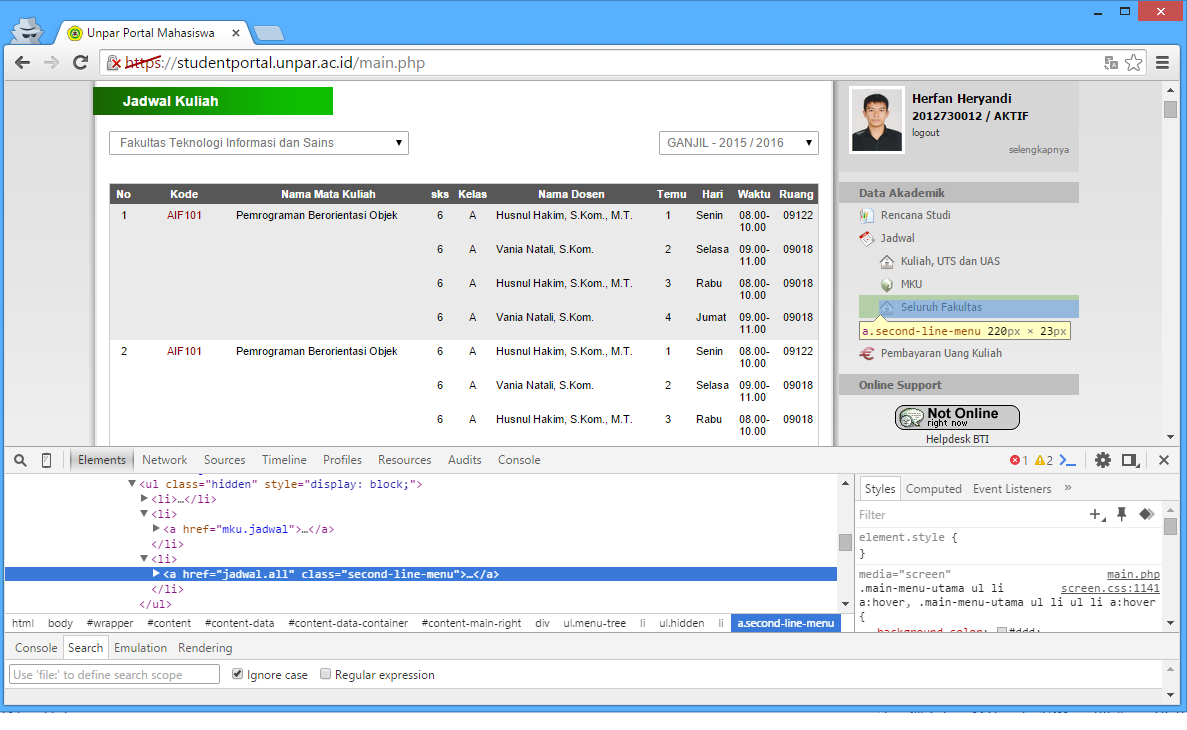
\includegraphics[scale=0.5]{Gambar/case-jadwal-seluruh}
			\caption{Elemen ``a'' dengan teks ``Seluruh Fakultas'' pada Menu Jadwal} 
			\label{fig:3_case_jadwal_seluruh}
		\end{figure}
	\item Setelah diklik, mahasiswa akan diarahkan ke \url{https://studentportal.unpar.ac.id/includes/jadwal.all.php} dengan \textit{cookie} sebagai berikut:
\begin{itemize}
	\item PHPSESSID: diambil dari \textit{cookie} yang di-\textit{set} saat pengalihan ke halaman utama
\end{itemize}
		\item Halaman ``Seluruh Fakultas'' menampilkan seluruh jadwal semester terkini pada fakultas tempat mahasiswa menempuh studi. Jika ingin melihat jadwal semester sebelumnya, mahasiswa dapat mengklik \textit{combo box} ``select\#tahun\_akd\_sec'' kemudian memilih ``option'' yang diinginkan. Jika ingin melihat jadwal fakultas lain, mahasiswa dapat mengklik \textit{combo box} ``select\#jadwal\_all\_ps'' kemudian memilih ``option'' fakultas yang diinginkan (Gambar \ref{fig:3_case_jadwal_pilihfak}).
		\begin{figure}[H]
			\centering
			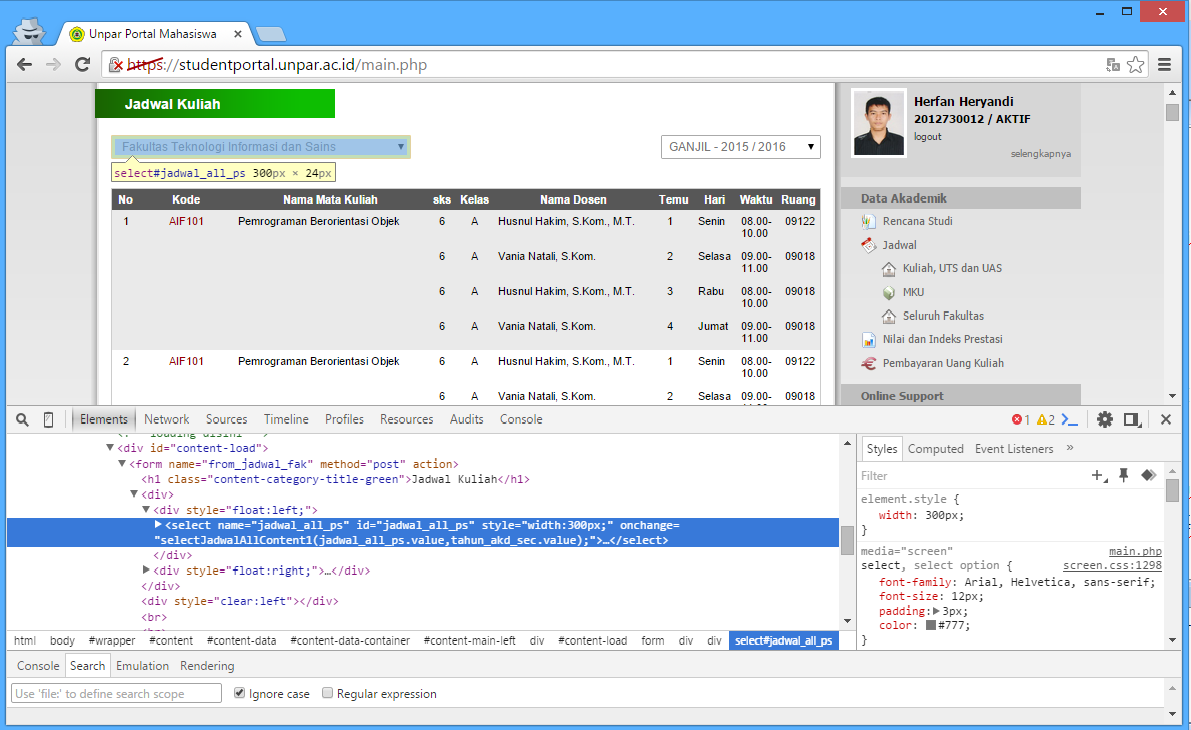
\includegraphics[scale=0.5]{Gambar/case-jadwal-pilihfak}
			\caption{Combo Box ``select\#jadwal\_all\_ps'' pada Halaman Jadwal Seluruh Fakultas} 
			\label{fig:3_case_jadwal_pilihfak}
		\end{figure}
		\item  Setelah memilih ``option'', mahasiswa akan dibawa ke \url{https://studentportal.unpar.ac.id/includes/jadwal.all.content.php}(Gambar \ref{fig:3_case_jadwal_fakultas}) dengan \textit{cookie} PHPSESSID dan mengandung \textit{query string parameter}:
		\begin{itemize}
			\item kode\_fak: berisi kode fakultas 
			\item thn\_akd: berisi tahun akademik semester 
			\item sem\_akd: berisi semester akademik dalam angka (1: ganjil, 2: genap, 4: pendek) 
		\end{itemize}
		
		\begin{figure}[H]
			\centering
			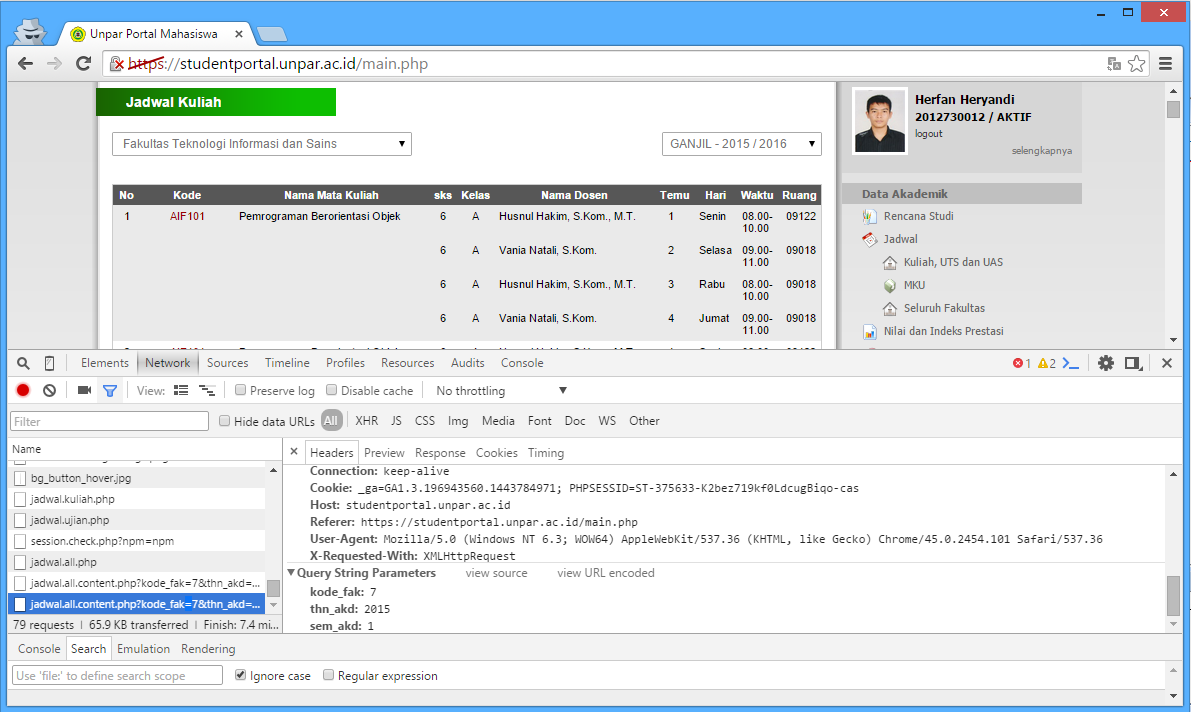
\includegraphics[scale=0.5]{Gambar/case-jadwal-fakultas}
			\caption{\textit{Form Data} pada pengiriman Jadwal Seluruh Fakultas} 
			\label{fig:3_case_jadwal_fakultas}
		\end{figure}
\end{enumerate}

\subsection{Kasus \textit{Logout}}
Mahasiswa dapat melakukan \textit{logout} dengan cara:
\begin{enumerate}
	\item Mengklik ``a'' dengan teks ``logout'' pada bagian identitas portal (Gambar \ref{fig:3_case_logout_link})
	\begin{figure}[H]
			\centering
			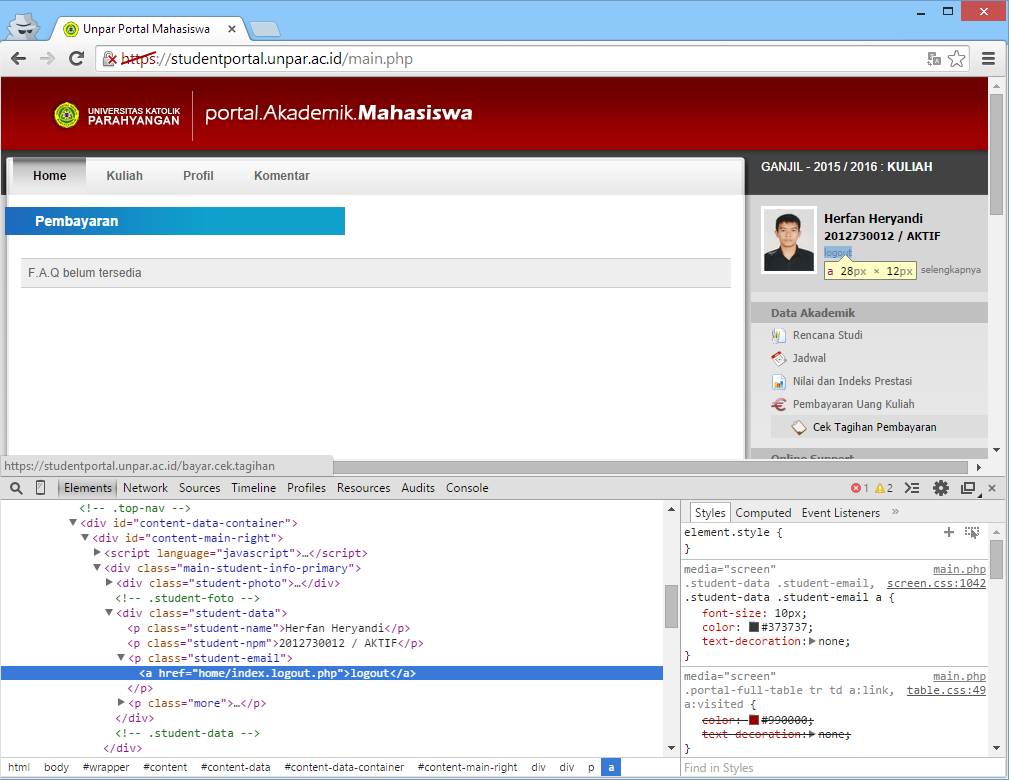
\includegraphics[scale=0.5]{Gambar/case-logout-link}
			\caption{Elemen ``a'' dengan teks ``logout'' pada Identitas Portal} 
			\label{fig:3_case_logout_link}
		\end{figure}
	\item Setelah diklik, mahasiswa akan diarahkan ke \url{https://studentportal.unpar.ac.id/home/index.logout.php} dengan \textit{cookie} sebagai berikut:
		\begin{itemize}
			\item PHPSESSID: diambil dari \textit{cookie} yang di-\textit{set} saat pengalihan ke halaman utama
		\end{itemize} 
	\item Kemudian dilakukan pengalihan ke \url{https://cas.unpar.ac.id/logout?service=https\%3A\%2F\%2Fstudentportal.unpar.ac.id} lalu mengadaluarsakan \textit{cookie} CASTGC dan CASPRIVACY yang sebelumnya di-\textit{set} saat pengalihan ke halaman utama (Gambar \ref{fig:3_case_logout_expires}) 
			\begin{figure}[H]
				\centering
				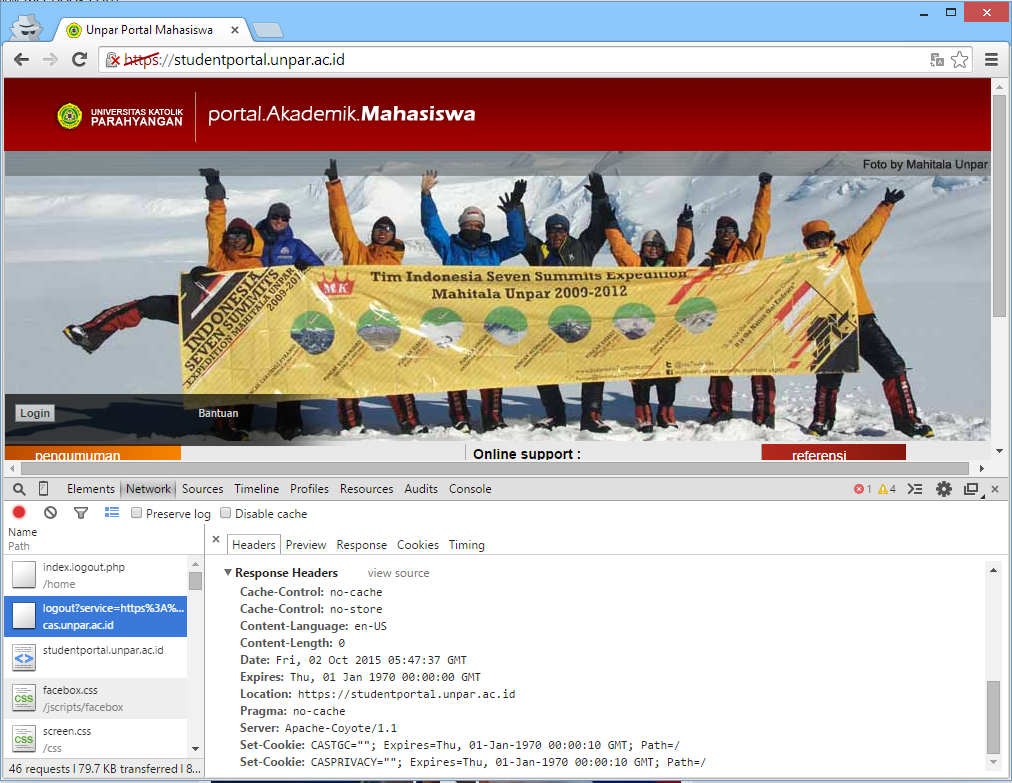
\includegraphics[scale=0.5]{Gambar/case-logout-expires}
				\caption{Pengadaluarsaan Cookie CASTGC dan CASPRIVACY} 
				\label{fig:3_case_logout_expires}
			\end{figure}
		\item Pengalihan diakhiri di \url{https://studentportal.unpar.ac.id/} yaitu halaman depan Portal Akademik Mahasiswa (Gambar \ref{fig:3_case_logout}) 
		\begin{figure}[H]
				\centering
				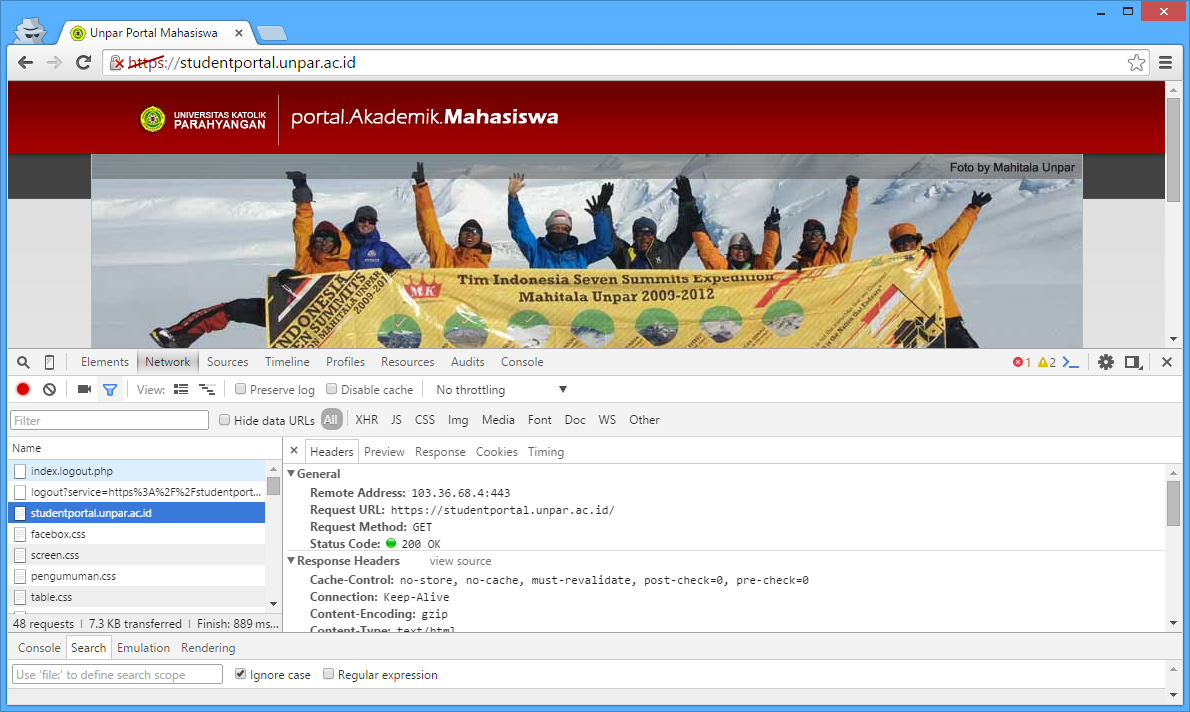
\includegraphics[scale=0.5]{Gambar/case-logout}
				\caption{Pengalihan ke Halaman Depan Portal Akademik Mahasiswa} 
				\label{fig:3_case_logout}
			\end{figure}
\end{enumerate}

Hasil analisis komunikasi Portal Akademik Mahasiswa akan digunakan untuk membangun koneksi yang akan diimplementasikan menggunakan jsoup. Berdasarkan hasil analisis tersebut, terdapat tiga hal yang perlu diperhatikan antara lain:
	\begin{itemize}
	\item Perpindahan halaman \\
		Saat pengguna melakukan suatu aksi seperti klik dan memilih \textit{option}, Portal Akademik Mahasiswa akan mengarahkan pengguna ke suatu halaman. Alamat dari halaman tersebut perlu diketahui untuk koneksi jsoup. Metode pengirimannya juga perlu diketahui. Dari seluruh halaman yang dianalisis, metode pengirimannya adalah \texttt{GET} kecuali halaman \textit{login} CAS UNPAR yang menggunakan metode POST.
	\item\textit{Cookie} \\
		Hal yang harus diperhatikan dalam penggunaan \textit{cookie} yaitu kapan suatu \textit{cookie} di-\textit{set} dan kapan \textit{cookie} tersebut dikirimkan. Jika suatu halaman memerlukan \textit{cookie} saat membangun koneksi, maka perlu diketahui kapan \textit{cookie} tersebut di-\textit{set} sehingga \textit{cookie} tersebut bisa diperoleh menggunakan jsoup. Pengiriman \textit{cookie} tersebut akan diimplementasikan dengan jsoup saat membangun koneksi ke suatu halaman yang memerlukan \textit{cookie} tersebut.
	\item Parameter\\
	Saat berpindah halaman, terkadang halaman tersebut membutuhkan parameter data. Dalam membangun koneksi, jsoup memerlukan juga memerlukan parameter data, karena itu perlu diketahui parameter data apa saja yang harus dilewatkan saat menuju suatu halaman.
\end{itemize}

\section{Analisis Arsitektur Informatika Student Portal}
Arsitektur Informatika Student Portal dapat dilihat pada Gambar \ref{fig:3_ars_portal}. \textit{Client} dapat mengakses Portal Akademik Mahasiswa dan Informatika Student Portal untuk mendapatkan informasi akademik. Namun saat mengakses Informatika Student Portal, \textit{client} akan diberikan data akademik dengan fitur-fitur yang berbeda. Saat \textit{client} mengakses Informatika Student Portal, Informatika Student Portal akan mengambil data dari Portal Akademik Mahasiswa. Data yang telah diambil akan diolah kemudian ditampilkan kepada \textit{client}.

		\begin{figure}[H]
			\centering
			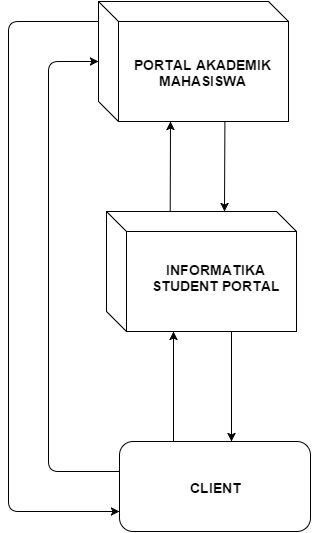
\includegraphics[scale=0.5]{Gambar/arsitekturIFPortal}
			\caption{Arsitektur Informatika Student Portal} 
			\label{fig:3_ars_portal}
		\end{figure}
		
\section{Analisis \textit{Use Case}}
\subsection{Diagram \textit{Use Case}}
Diagram \textit{use case} pada perangkat lunak yang akan dibangun hanya mengandung satu aktor, yaitu mahasiswa. Diagram \textit{use case} dapat dilihat pada gambar \ref{fig:3_usecase_diagram}. 
		\begin{figure}[H]
			\centering
			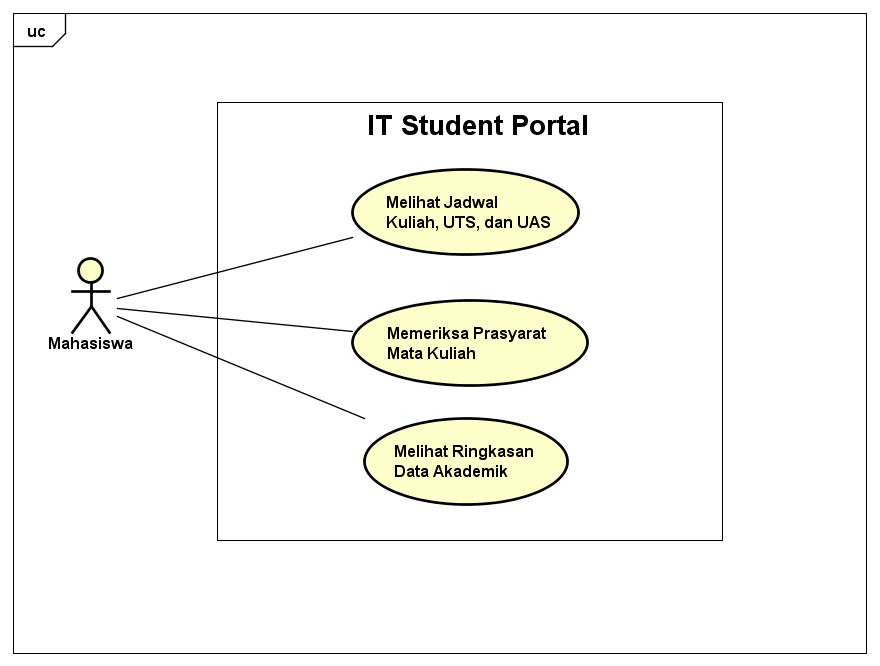
\includegraphics[scale=0.5]{Gambar/usecase-diagram}
			\caption{Diagram \textit{Use Case} Informatika Student Portal} 
			\label{fig:3_usecase_diagram}
		\end{figure}
Berdasarkan hasil analisis pada subbab \ref{sec:kebutuhan}, dari lima fitur yang akan dibuat, dibentuk tiga \textit{use case} antara lain:
\begin{itemize}
	\item \textbf{Memeriksa Prasyarat Mata Kuliah}, mahasiswa dapat memeriksa mata kuliah yang dibuka pada semester terkini apakah memenuhi prasyarat atau tidak. 
	\item \textbf{Melihat Jadwal Kuliah}, mahasiswa dapat melihat jadwal kuliah yang sudah tersusun dan terurut berdasarkan hari.
	\item \textbf{Melihat Ringkasan Data Akademik}, mahasiswa dapat melihat data mengenai mata kuliah apa saja yang sudah lulus beserta jenis mata kuliahnya(wajib, pilihan, atau pilihan wajib), sisa SKS untuk mencapai kelulusan, dan mata kuliah wajib yang belum ditempuh. Mahasiswa juga dapat melihat IPS dan IPK yang berubah berdasarkan riwayat nilai.
\end{itemize}

\subsection{Skenario \textit{Use Case}}

\begin{enumerate}
	\item \textbf{Memeriksa Prasyarat Mata Kuliah}
		\begin{itemize}
			\item Nama: Memeriksa prasyarat mata kuliah
			\item Aktor: Mahasiswa
			\item Deskripsi: Memeriksa prasyarat mata kuliah yang dibuka pada semester terkini
			\item Kondisi awal: Mahasiswa telah \textit{login}
			\item Kondisi akhir: Halaman prasyarat mata kuliah ditampilkan dan berisi prasyarat mata kuliah yang dibuka pada semester terkini
			\item Skenario utama: \\ \\
				\begin{tabular}{|p{0.5cm} |p{6cm}| p{6cm}|}
						\hline
							No 	& Aksi Aktor & Reaksi Sistem \\ \hline
							1 	& Mahasiswa memilih menu prasyarat mata kuliah. 	&	Sistem mendapatkan data mahasiswa kemudian menampilkan halaman prasyarat mata kuliah \\ \hline 
						\end{tabular} 
			\item Eksepsi: Mahasiswa sedang menempuh semester 1
		\end{itemize}
		
	\item \textbf{Melihat Jadwal Kuliah}
		\begin{itemize}
			\item Nama: Melihat jadwal kuliah
			\item Aktor: Mahasiswa
			\item Deskripsi: Melihat jadwal kuliah yang sudah tersusun dan terurut berdasarkan hari
			\item Kondisi awal: Mahasiswa telah \textit{login}
			\item Kondisi akhir: Halaman jadwal ditampilkan dan berisi jadwal kuliah, UTS, dan UAS yang sudah tersusun dan terurut berdasarkan hari te
			\item Skenario utama: \\ \\
				\begin{tabular}{|p{0.5cm} |p{6cm}| p{6cm}|}
						\hline
							No 	& Aksi Aktor & Reaksi Sistem \\ \hline
							1 	& Mahasiswa memilih menu jadwal. 	&	Sistem menyusun dan mengurutkan jadwal mahasiswa berdasarkan hari kemudian menampilkan halaman jadwal \\ \hline 
						\end{tabular} 
			\item Eksepsi: Mahasiswa sedang cuti studi atau jadwal kuliah belum keluar
		\end{itemize}
		
	\item \textbf{Melihat Ringkasan Data Akademik}
		\begin{itemize}
			\item Nama: Melihat ringkasan data akademik
			\item Aktor: Mahasiswa
			\item Deskripsi: melihat data mengenai mata kuliah apa saja yang sudah lulus beserta jenis mata kuliahnya(wajib, pilihan, atau pilihan wajib), sisa SKS untuk mencapai kelulusan, dan mata kuliah wajib yang belum ditempuh. Mahasiswa juga dapat melihat IPS dan IPK yang berubah berdasarkan riwayat nilai
			\item Kondisi awal: Mahasiswa telah \textit{login}
			\item Kondisi akhir: Halaman jadwal ditampilkan dan berisi jadwal ringkasan data akademik
			\item Skenario utama: \\ \\
			\begin{tabular}{|p{0.5cm} |p{6cm}| p{6cm}|}
						\hline
							No 	& Aksi Aktor & Reaksi Sistem \\ \hline
							1 	& Mahasiswa memilih menu ringkasan data akademik. 	&	Sistem meringkas data kademik mahasiswa kemudian menampilkan halaman ringkasan data akademik \\ \hline 
						\end{tabular} 
			\item Eksepsi: Mahasiswa sedang menempuh semester 1
		\end{itemize}
\end{enumerate}

\section{Analisis Kelas}
Diagram kelas analisis untuk Informatika Student Portal ditunjukkan pada gambar \ref{fig:3_class_diagram}.
	\begin{figure}[H]
			\centering
			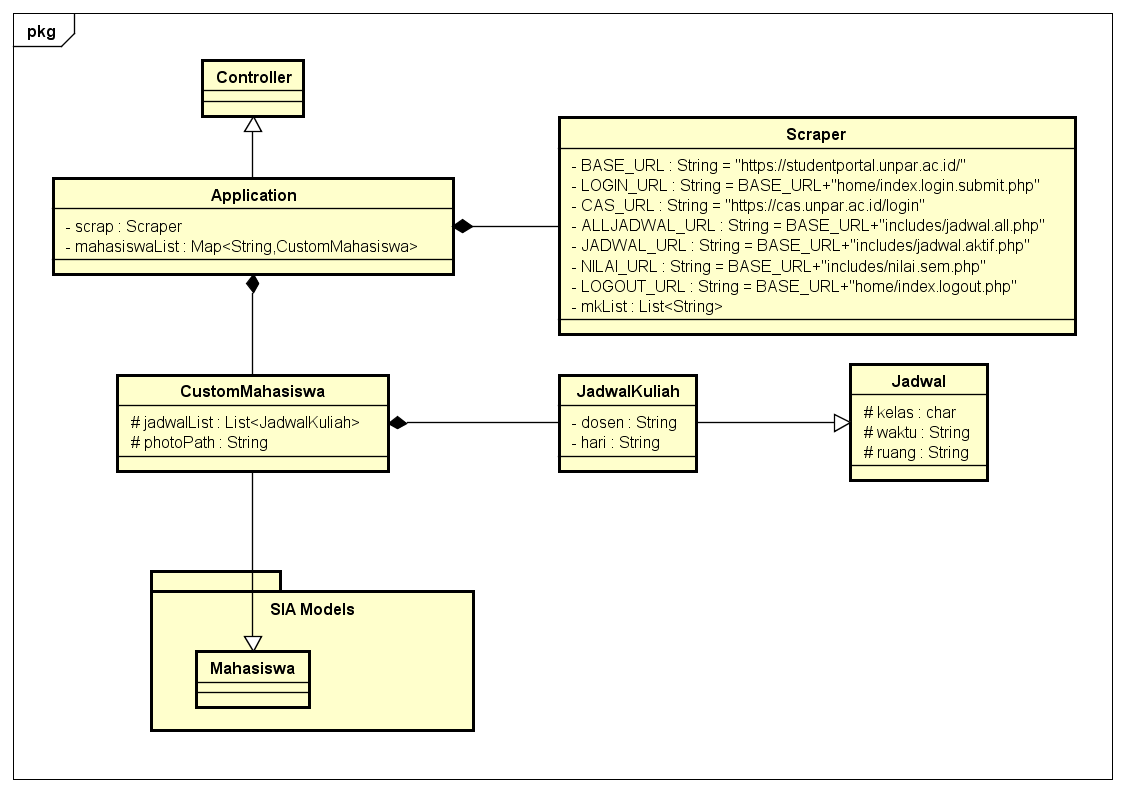
\includegraphics[scale=0.5]{Gambar/class-diagram}
			\caption{Diagram Kelas Analisis Informatika Student Portal} 
			\label{fig:3_class_diagram}
		\end{figure}
Kelas-kelas dari \textit{package} SIA Models telah dibahas pada subbab \ref{sec:siamodels}. Sedangkan penjelasan dari kelas-kelas lainnya sebagai berikut:
\begin{enumerate}
	\item Controller\\
	Kelas ini merupakan kelas yang sudah disediakan oleh Play Framework. Turunan dari kelas ini akan berperan sebagai \textit{controller}.
	\item Application\\
	Kelas ini merupakan \textit{controller} pada Informatika Student Portal yang berfungsi untuk menghubungkan \textit{model} dengan \textit{view}. 
	\item Scraper\\
	Kelas ini merupakan kelas yang mengimplementasikan \textit{web scraping} menggunakan \textit{library} jsoup. Kelas ini digunakan untuk memperoleh data dari Portal Akademik Mahasiswa kemudian menghubungkannya ke dalam SIA Models. Data-data yang sudah dihubungkan dengan SIA Models akan ditampilkan ke \textit{view} melalui kelas \texttt{Application}.
\end{enumerate}
		